\documentclass[11pt]{article}

\usepackage[a4paper,margin=2.3cm]{geometry}
\usepackage{graphicx}
\usepackage{booktabs}
\usepackage{amsmath}
\usepackage{hyperref}
\usepackage{xcolor}
\usepackage{caption}
\usepackage{titlesec}
\usepackage{authblk}
\usepackage{setspace}
\usepackage[numbers,sort&compress]{natbib}

\hypersetup{colorlinks=true, linkcolor=blue!45!black, urlcolor=blue!45!black, citecolor=blue!45!black}
\captionsetup{font=small, labelfont=bf}
\titleformat{\section}{\normalfont\large\bfseries}{\thesection.}{0.5em}{}
\titleformat{\subsection}{\normalfont\bfseries}{\thesubsection.}{0.5em}{}
\onehalfspacing

\title{\textbf{Probabilistic dengue and chikungunya forecasting in Brazil:\\
metric-dependent model rankings, regime-shift fragility, and conformal ensembles}}
\author[1]{Md Kamruzzaman Kamrul}
\author[2]{Eashraque Jahan Easha}
\author[3]{Abdullah Al Helal}
\affil[1]{Purdue University, West Lafayette, IN, USA}
\affil[2]{University of Denver, Denver, CO, USA}
\affil[3]{Oklahoma State University, Stillwater, OK, USA}
\date{\today}

\begin{document}
\maketitle

\begin{abstract}
\noindent
Dengue is expanding across Brazil, and 2024 produced a record epidemic of roughly four times any
prior year. Accurate, well-calibrated probabilistic forecasts support preparedness, but the
relative merits of statistical, machine-learning, deep-learning, and mechanistic approaches for
this task are unsettled, especially under the distribution shift an outbreak year imposes. We
report a reproducible, leakage-controlled comparison of five probabilistic forecasting model
families for the 3rd Infodengue--Mosqlimate Dengue Challenge (IMDC 2026), which requires weekly,
state-level forecasts with full predictive intervals for the 26 mandatory Brazilian states. All
models are evaluated through a single backtesting harness over four official retrospective seasons,
one of which contains the 2024 outbreak, and scored by the weighted interval score (WIS). We report
four results with implications beyond this challenge. First, no model is best across seasons: a
global recurrent network is the most accurate model in normal seasons yet the worst on the 2024
outlier, whereas an ensemble never incurs any member's worst-season failure. Second, the identity
of the best model depends on the evaluation metric, because magnitude-weighted mean WIS and
scale-free normalized WIS reward accuracy on different subsets of a highly skewed set of states.
Third, a conformal recalibration, a post-hoc widening of the ensemble's prediction intervals by a
factor tuned to fix their overconfidence, improves accuracy and calibration at negligible cost
(mean WIS, a magnitude-weighted score, 1234 to 1162; normalized WIS, its scale-free counterpart,
0.595 to 0.561; out-of-sample reduction of 6.2 percent). It acts as asymmetric insurance: the
extra interval width costs little in an ordinary season but prevents the catastrophic under-prediction
an extreme season would otherwise cause. Fourth, added
model complexity did not pay: observed-climate covariates and hierarchical spatial pooling both
failed to improve forecasts, and an internal-holdout hyperparameter gain reversed on the true
backtest. The best model is disease-specific: for chikungunya, gradient boosting alone outperforms
the ensemble. All code, the backtesting harness, per-state scored predictions, and validated
submissions for four official tracks are released, with an automated test suite covering leakage,
scoring, and every model.
\end{abstract}

\section*{Author summary}
\noindent
Brazil carries one of the world's largest dengue burdens, and 2024 brought an epidemic without
precedent in the national record. Public-health agencies increasingly rely on forecasts that state
not just a single predicted number of cases but a full range of plausible outcomes with calibrated
uncertainty. Which forecasting method to trust is an open question, particularly during an
exceptional season when accurate forecasts matter most. We compared five families of models,
ranging from simple seasonal baselines to gradient boosting, deep learning, and a mechanistic
epidemic model, on identical retrospective tests across four dengue seasons in all 26 mandatory
Brazilian states. We found that no method is best everywhere: the deep-learning model was the most
accurate in ordinary seasons but failed badly during the 2024 outbreak, while a simple ensemble
that averages the models was the most dependable. We also found that the apparent winner changes
depending on how performance is scored, a caution for forecasting leaderboards. Finally, a light
statistical recalibration that stretched the ensemble's prediction intervals just enough to fix
them being too narrow improved both accuracy and reliability, and
adding more data or model complexity did not help. At the challenge's own validation-round results
presentation, our submission was independently named one of six best-overall-performing models (of
27 submitted) for the mandatory state-level dengue target, and one of three models with outstanding
performance on the optional city-level target \citep{imdc2026webinar}. Our full pipeline is openly
available.

\section{Introduction}
Dengue is among the fastest-spreading mosquito-borne diseases, with an estimated 390 million
infections each year and roughly half of the world's population at risk, a range that continues to
expand with climate change and urbanization \citep{bhatt2013,messina2019,colon2021}. Brazil bears one
of the largest national burdens \citep{lowe2021}. The 2024 season broke the national record by a wide
margin, with a peak of 451{,}578 reported cases in a single epidemiological week and an annual total
near 6.67 million, roughly four times the next-largest year on record. Transmission is shaped by
climate, and the 2023--24 El Ni\~no is one of several drivers implicated in the surge. Against this
background, arboviral forecasting has moved from point prediction toward full probabilistic
forecasts, motivated by the recognition that preparedness decisions depend on the entire predictive
distribution rather than a single expected value \citep{gneiting2014,johansson2019,cramer2022}.

The Infodengue--Mosqlimate Dengue Challenge (IMDC) operationalizes this shift. It invites teams to
submit weekly, state-level probabilistic forecasts with prescribed quantiles, scored by the weighted
interval score, following the precedent of the inaugural 2024 edition \citep{araujo2026}. The
challenge exposes a question that the wider forecasting literature has not resolved for this
setting: given statistical, machine-learning (ML), deep-learning (DL), and mechanistic approaches,
which forecast best, and how robustly, when a season can depart by an order of magnitude from
anything in the training record?

We address this with a controlled comparison built for reproducibility and for honest evaluation
under distribution shift. Every model is fit and scored through one backtesting harness that
enforces leakage safety and applies the same scoring code to all forecasts, over the four official
retrospective seasons (2022--23 through 2025--26) for the 26 mandatory states. We make the following
contributions.

\begin{enumerate}
\item We show that model rankings are season-dependent and, in the outbreak year, invert: the model
that is best on average can be the least reliable exactly when reliability matters most
(Section~\ref{sec:noseason}).
\item We show that the identity of the best model depends on whether skill is weighted by case
magnitude or by forecasting unit, a consequence of real cross-state heterogeneity rather than an
artifact, and we argue for reporting both (Section~\ref{sec:metric}).
\item We introduce a conformal recalibration of the ensemble intervals that improves accuracy and
calibration at negligible cost and functions as asymmetric insurance against catastrophic
under-prediction (Section~\ref{sec:conformal}).
\item We document informative negative results: added covariates, hierarchical pooling,
hyperparameter tuning, and an alternative ensemble-combination rule each failed to improve
forecasts where it mattered most, which clarifies where the predictable signal in this problem
lies (Section~\ref{sec:negative}).
\item We show that the best model is disease-specific, using chikungunya as a contrasting target
(Section~\ref{sec:chik}), and we release the complete, tested pipeline.
\end{enumerate}

\section{Results}

\subsection{Study design and data}\label{sec:design}
We forecast weekly dengue case counts per state across the 2022--23 through 2025--26 seasons for the
26 mandatory Brazilian states (Espírito Santo is excluded per the challenge specification). These
four seasons are referred to throughout as folds 1 through 4 (fold 1: 2022--23; fold 2: 2023--24,
containing the 2024 outbreak; fold 3: 2024--25; fold 4: 2025--26, partially resolved). Each fold is
defined by an official training cutoff, the last date a model fitted for that fold is allowed to
see, and a target window, the season it must forecast; a confirmed
15-week gap separates each training cutoff from the start of its evaluation window, reflecting the
reporting delay a real forecaster faces (Fig~\ref{fig:overview}). Forecasts are submitted as nine
quantiles per state and week, from which the four central prediction intervals (50, 80, 90, and 95
percent) are formed. All covariate access, feature construction, and model fitting are filtered to
data at or before each training cutoff, and this discipline is enforced by automated tests rather
than by convention (Section~\ref{sec:methods}). The four seasons differ by an order of magnitude in
difficulty. The 2023--24 season (fold 2), which contains the 2024 outbreak, is the hardest for every
model, and the 2025--26 season (fold 4) is only partially resolved in the available data and is
reported separately.

\begin{figure}[t]
\centering
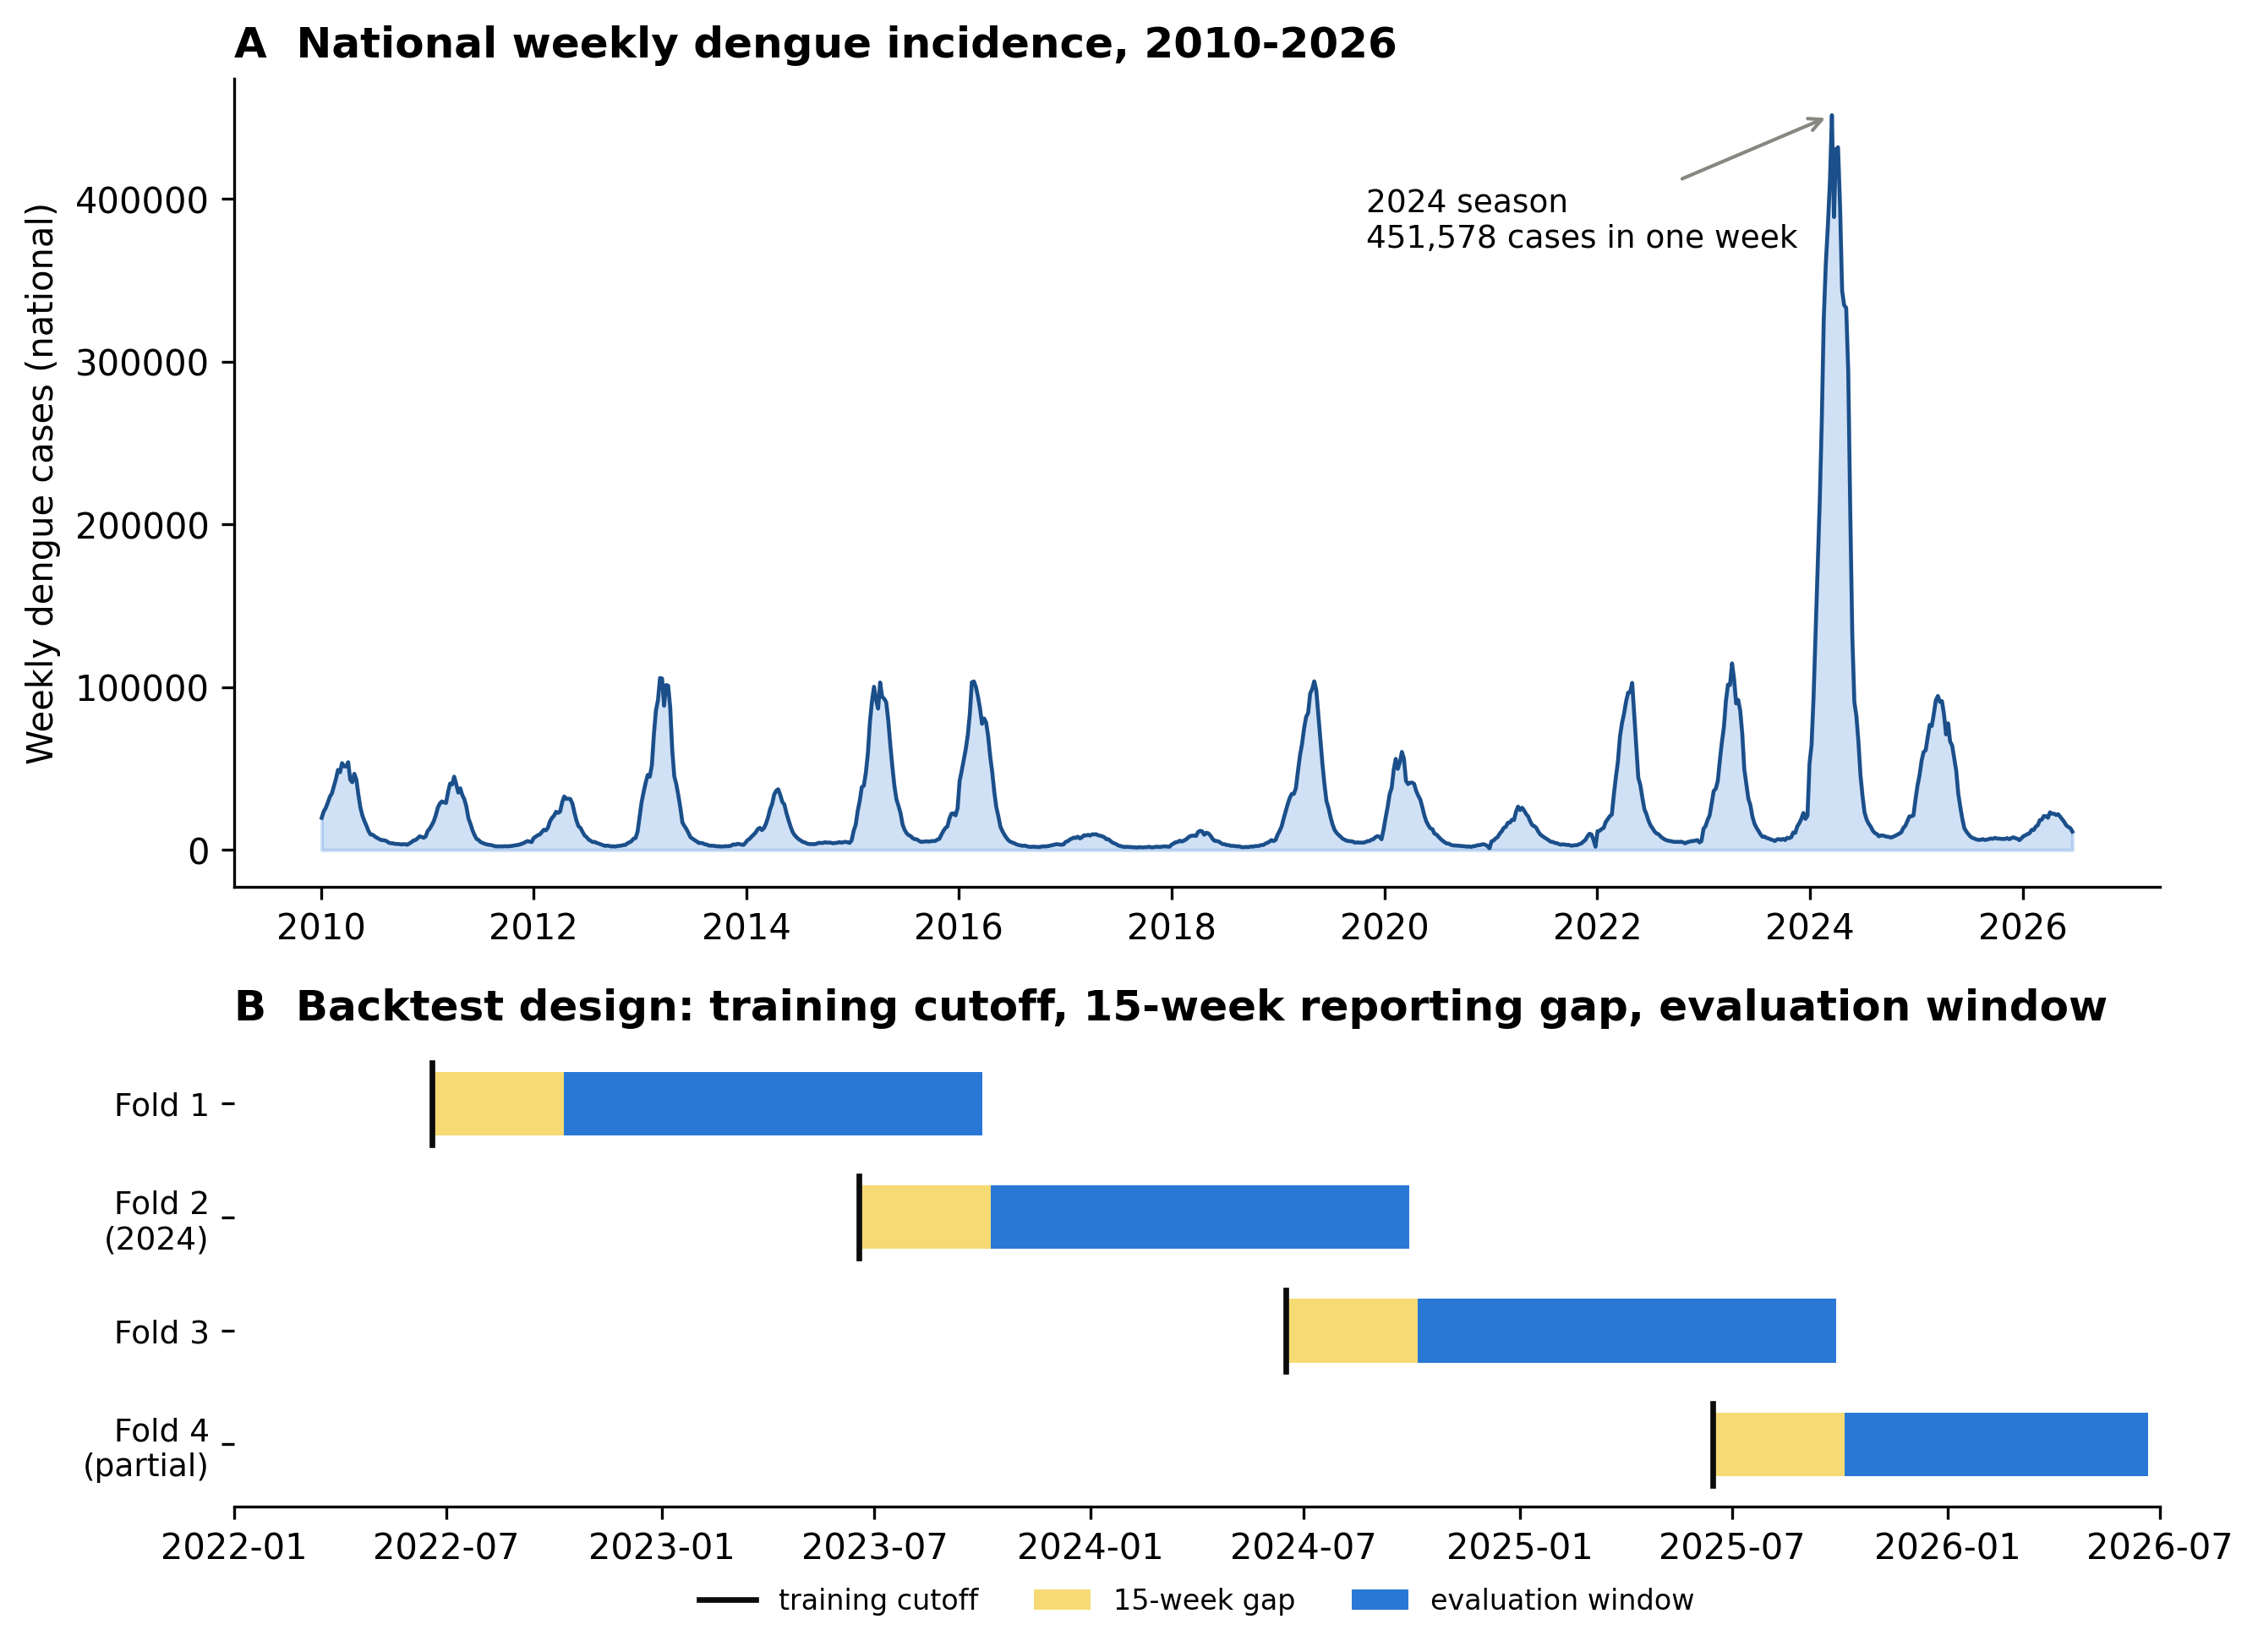
\includegraphics[width=0.95\textwidth]{../results/figures/paper_design.png}
\caption{\textbf{Data and study design.} (A) Weekly reported dengue cases aggregated to the national
level, 2010--2026; the 2024 season stands roughly four times above any prior year. (B) The four
official retrospective seasons form a rolling backtest. Each has a training cutoff (all data up to
the cutoff is used for fitting), a 15-week reporting gap, and an evaluation window on which forecasts
are scored. Fold 2 covers the 2024 outbreak and fold 4 is partially resolved.}
\label{fig:overview}
\end{figure}

\subsection{No single model dominates across seasons}\label{sec:noseason}
Table~\ref{tab:byfold} reports mean WIS by model and season, and Fig~\ref{fig:byfold} shows the same
on a log scale. The ranking of models reorders across seasons. The deep network (a global GRU with a
negative-binomial head, an output layer suited to over-dispersed count data such as case counts,
rather than the Poisson head more common in count models) is the single best model in the two
ordinary seasons, folds 1 and 3 (WIS 348 and 324), but is the worst of all models on the 2024
outlier, fold 2 (WIS 4131), worse even than a naive baseline, because the surge lies outside its
training distribution and its intervals, derived from its fitted distribution rather than built
empirically, are too narrow to cover it. The gradient-boosted model (XGBoost, chosen over a second
gradient-boosting implementation, LightGBM, that we also tested and that scored significantly worse
overall, Section~\ref{sec:methods}) is the strongest single model on the outlier season (WIS 3238),
but unlike LightGBM, which showed a sharper trade-off (strongest on the outlier at WIS 3332 yet the
weakest of the serious models on the ordinary season fold 3, WIS 665), XGBoost remains reasonably
competitive rather than collapsing in the ordinary seasons (WIS 376 and 484 in folds 1 and 3). The
semi-mechanistic trajectory model is near best on the outlier (WIS 3371)
because its bootstrap of historical seasons yields wide intervals precisely when they are needed.
This season-dependence is the central obstacle the challenge poses: a model selected on average
performance carries a hidden risk of catastrophic failure in the season that matters most.

\begin{table}[t]
\centering\small
\caption{\textbf{Dengue mean WIS by season (fold).} Lower is better. Fold 2 contains the 2024
outbreak and is roughly ten times harder than any other season. Fold 4 (2025--26) is partially
resolved and reported separately. Best value in each column is in bold.}
\label{tab:byfold}
\begin{tabular}{@{}lrrrr@{}}
\toprule
\textbf{Model} & \textbf{Fold 1} & \textbf{Fold 2} & \textbf{Fold 3} & \textbf{Fold 4} \\
& 2022--23 & 2023--24 & 2024--25 & 2025--26 \\
\midrule
Ensemble (conformal)      & 337 & 3297 & 403 & 408 \\
Ensemble (Vincentization) & 338 & 3574 & 398 & 399 \\
Ensemble (inverse-WIS)    & \textbf{313} & 3625 & \textbf{387} & 401 \\
GRU (deep learning)       & 348 & 4131 & \textbf{324} & 542 \\
XGBoost                   & 376 & \textbf{3238} & 484 & 468 \\
Mechanistic               & 468 & 3371 & 551 & 314 \\
Climatological            & 386 & 3588 & 516 & 309 \\
Seasonal-naive            & 500 & 3848 & 581 & 293 \\
Naive                     & 726 & 3833 & 1056 & \textbf{266} \\
\bottomrule
\end{tabular}
\end{table}

\begin{figure}[t]
\centering
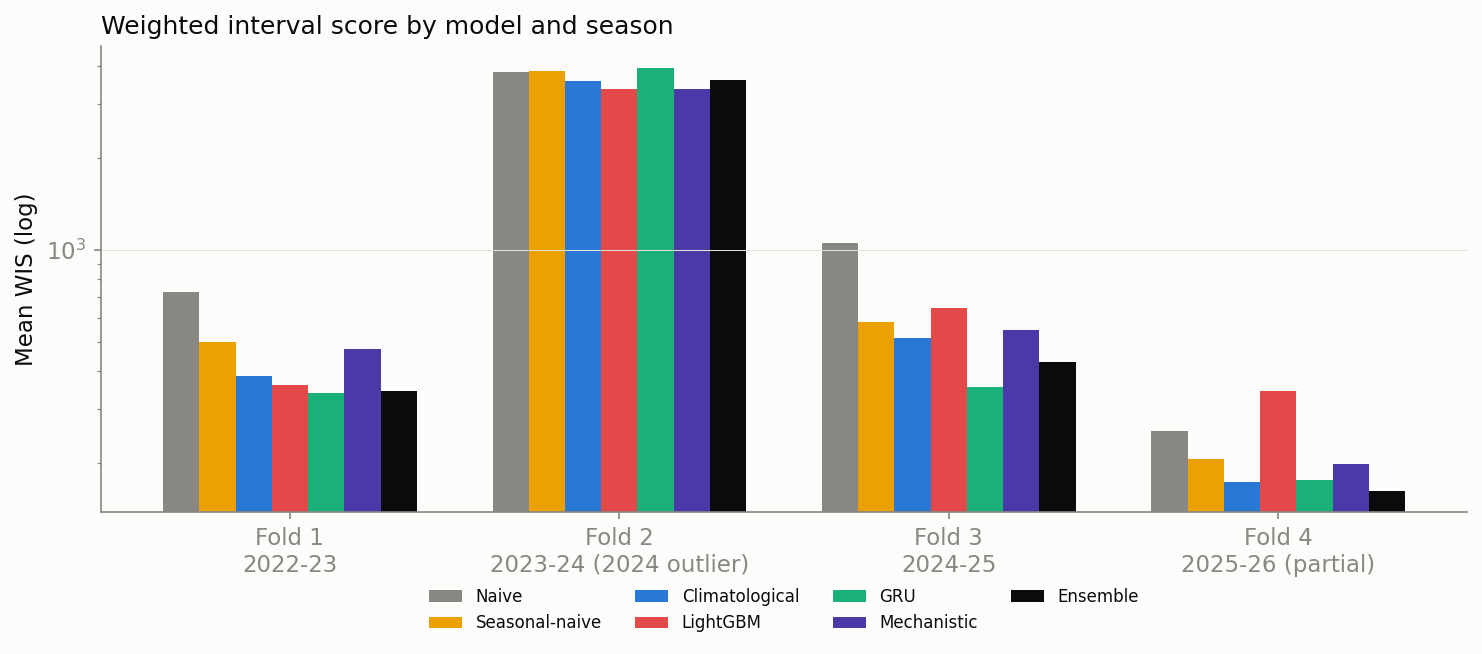
\includegraphics[width=0.72\textwidth]{../results/figures/paper_wis_by_fold.png}
\caption{\textbf{Mean WIS by model and season (log scale).} Model rankings reorder across seasons.
The deep network is best in ordinary seasons and worst on the 2024 outlier; the ensemble avoids
every model's worst-season failure. The conformal-recalibrated ensemble (Section~\ref{sec:conformal})
is shown alongside its members.}
\label{fig:byfold}
\end{figure}

Season-to-season stability is a distinct axis from mean skill, and the two disagree for the models
identified above. For each fold we compute each model's relative WIS against the seasonal-naive
baseline (a fully-crossed pairwise comparison over state and horizon, Cramer et al. 2022), take its
log so that a model twice as good and a model twice as bad are symmetric, and summarize the four
folds by their mean (overall skill against the baseline, negative is better) and standard deviation
(season-to-season consistency, lower is more stable). Fig~\ref{fig:stability} plots the two against
each other. A log relative WIS of $-0.42$, for instance, means a model whose WIS is on average
$e^{0.42}\approx1.5$ times smaller than the baseline's, i.e. about 1.5 times more accurate; a
positive value of the same size would mean 1.5 times worse. The deep network has the best mean
skill of any model on this scale ($-0.42$) but
also the highest variability of any model except naive ($0.24$), the quantitative signature of its
ordinary-season strength and outlier-season failure. The mechanistic model sits at the opposite
corner: modest mean skill ($-0.09$) but the lowest variability of any model ($0.04$), because its
bootstrap of historical seasons widens intervals in proportion to historical variability rather than
assuming a fixed noise scale. Both ensembles trade part of the deep network's mean skill for
markedly better consistency (std $0.15$ and $0.13$ for the median and conformal ensembles), which is
the quantitative counterpart of the qualitative claim above: an ensemble is not chosen for being the
single best model in any one season, but for never being the worst.

\begin{figure}[t]
\centering
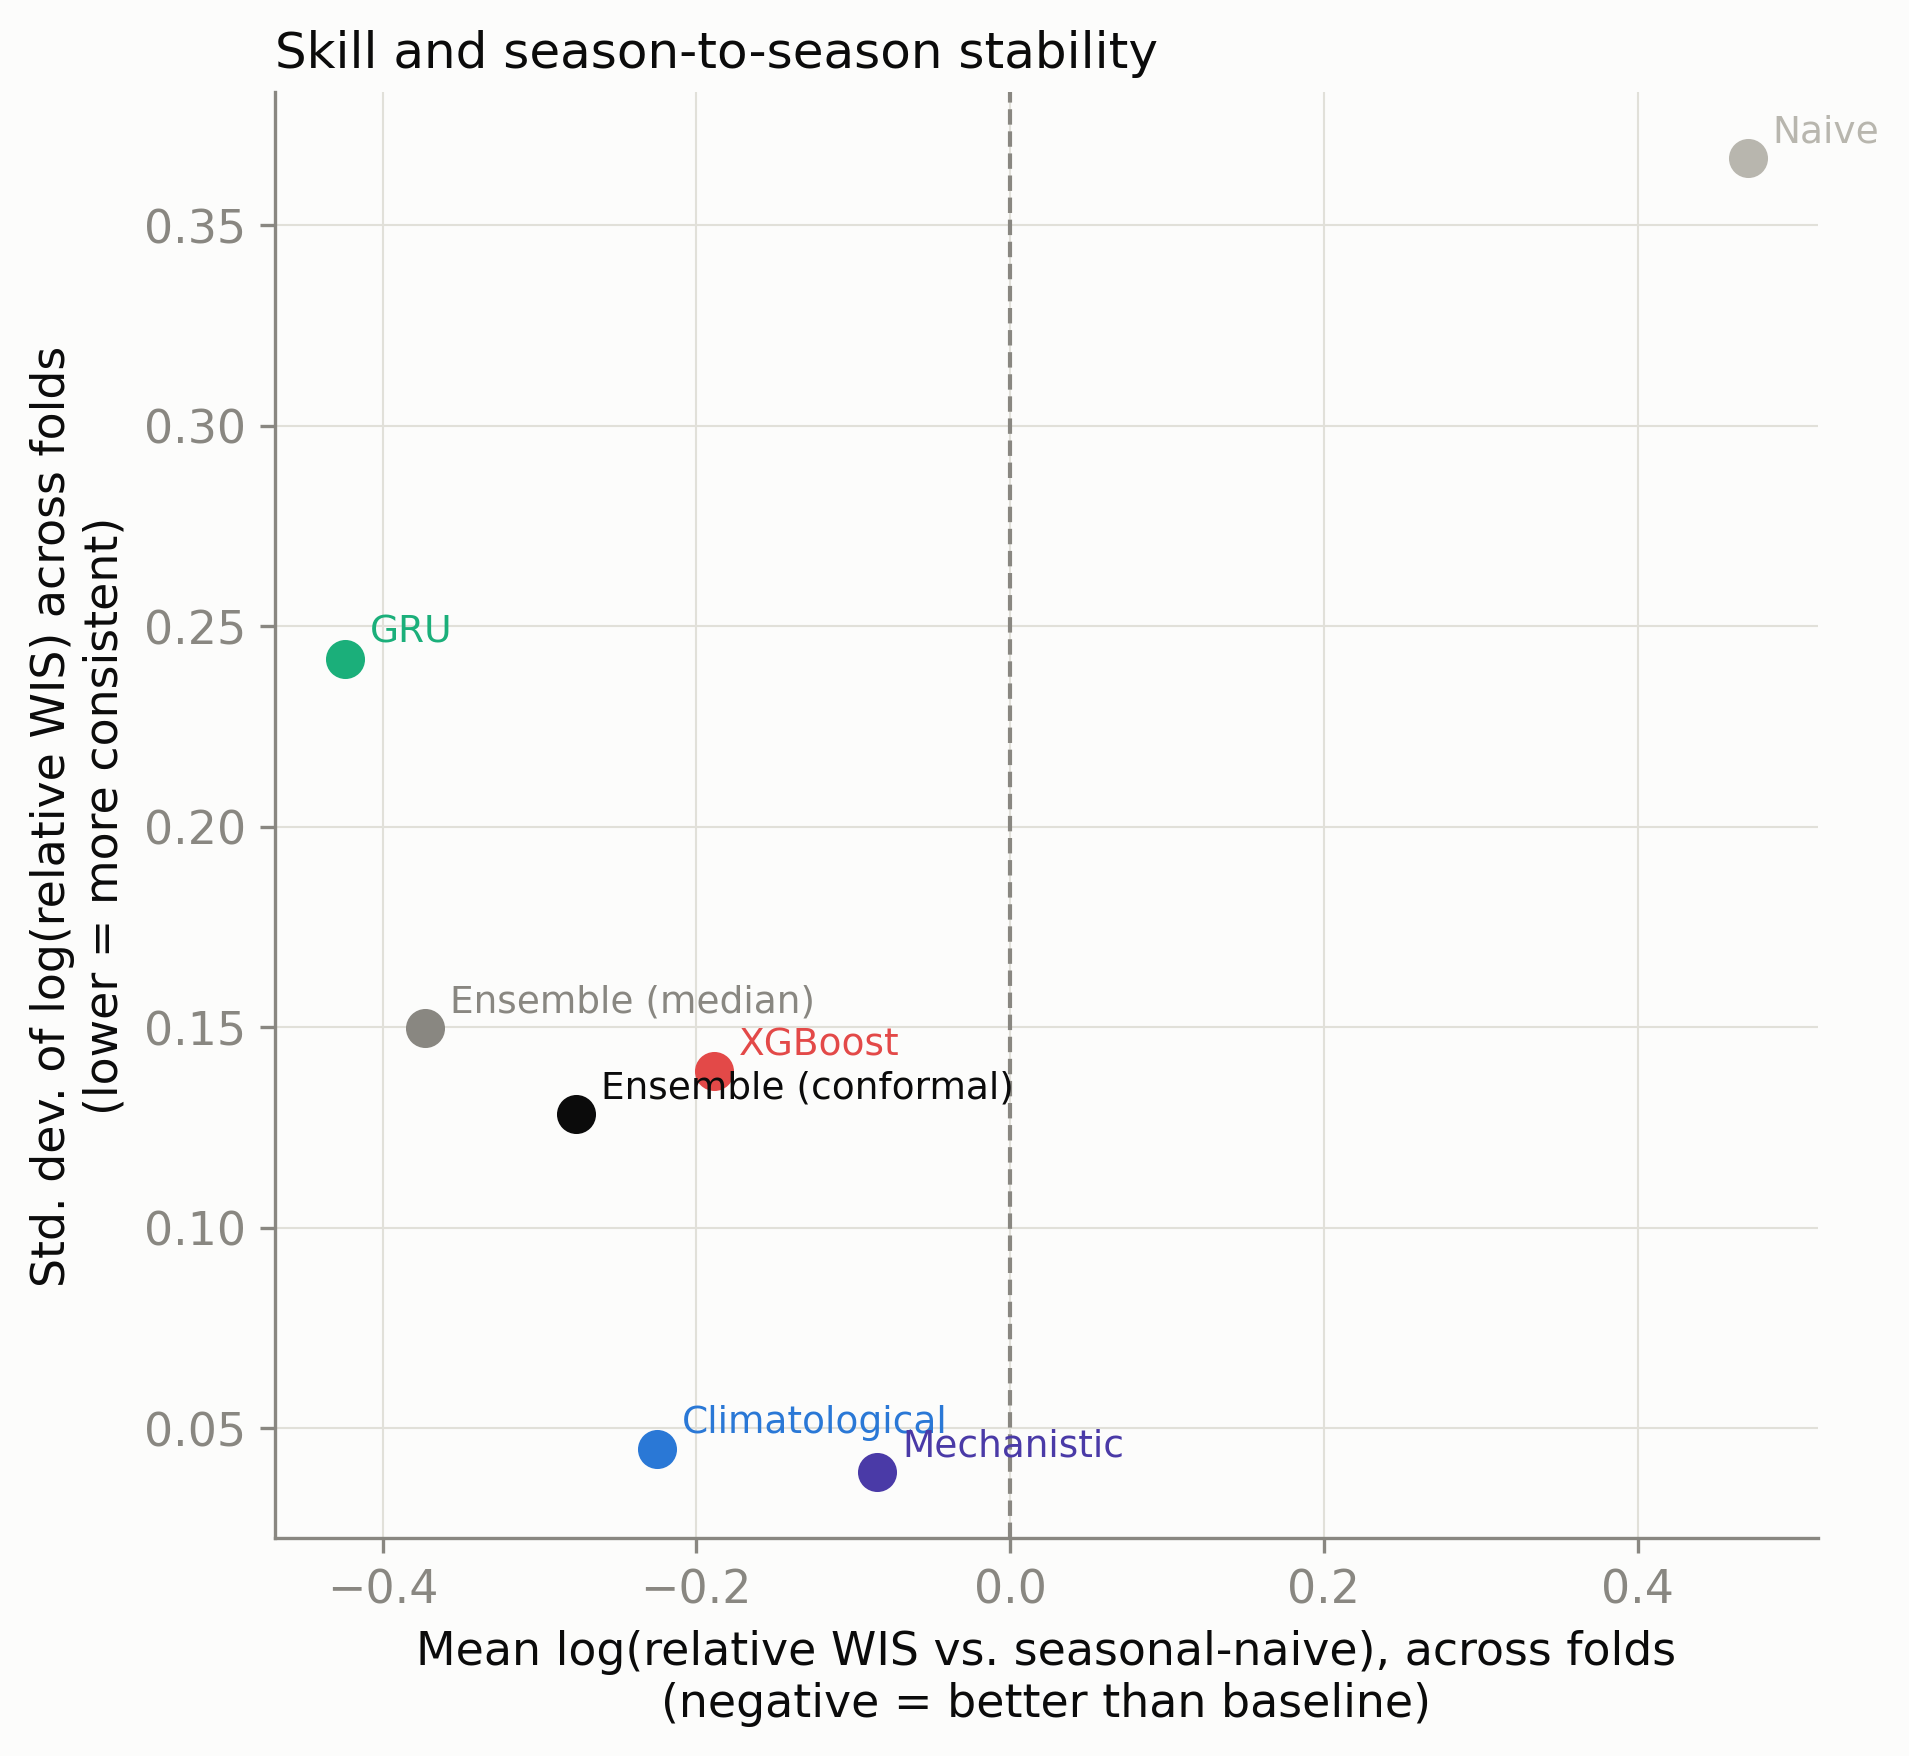
\includegraphics[width=0.62\textwidth]{../results/figures/paper_stability.png}
\caption{\textbf{Skill and season-to-season stability are distinct axes.} Each point is one model's
mean log relative WIS against the seasonal-naive baseline across the four folds (x, negative is
better) against the standard deviation of that same quantity (y, lower is more consistent). The deep
network has the best mean skill but is among the least stable; the mechanistic model is the most
stable but has only modest mean skill; the ensembles occupy an intermediate position that no single
member reaches.}
\label{fig:stability}
\end{figure}

\subsection{An ensemble is the most robust model, and conformal recalibration makes it the most
accurate}\label{sec:conformal}
Because different models win different seasons, a combination that is never worst is attractive. An
unweighted per-quantile median ensemble, Vincentization, meaning that at every quantile level (the
median, the 2.5th percentile, and so on) we take the median of the three models' values at that
level, of the climatological, gradient-boosted (XGBoost),
and deep-learning models avoids the catastrophic single-season failure of its weakest member
(WIS 3574 in the outlier season, far below the deep network's 4131) but, once XGBoost replaced a
weaker gradient-boosted alternative as the strongest single model (Section~\ref{sec:methods}), no
longer beats that single model outright on raw WIS alone (1234 versus 1190 for XGBoost;
Table~\ref{tab:leaderboard}). Its interval calibration is close to nominal but slightly narrow.

We improve on it with a conformal recalibration of the ensemble intervals, a distinct step from the
conformalized quantile regression (CQR) used inside the gradient-boosted model
(Section~\ref{sec:methods-conformal}
gives the full procedure): both stretch prediction intervals to fix them being too narrow, but CQR
calibrates one model's own intervals during fitting, whereas this step recalibrates the already-combined
ensemble's intervals afterward. Calibration factors that make each central interval reach its
nominal coverage are estimated on a single tuning season (fold 1) and applied to all seasons. The
estimated factors are gentle and concentrate on the tails: 1.08, 1.04, 1.19, and 1.86 for the 50,
80, 90, and 95 percent intervals. Concretely, a raw 95 percent interval of, say, [40, 160] around a
median of 100 becomes approximately [$-12$, 212], clipped to [0, 212] for non-negativity, after the
1.86 factor: the median is never touched, only the interval stretches, and it stretches only where
it needs to (the 80 percent interval above needed only a negligible correction). This step is what
turns the ensemble into the single best model overall, not merely a hedge against any one member's
worst case: the recalibrated ensemble is the most accurate model overall
(mean WIS 1162 versus 1234 for the plain ensemble and versus 1190 for the best single model,
XGBoost; normalized WIS 0.561 versus 0.595) and better
calibrated at the tails (empirical coverage 46/74/87/94 versus 43/72/82/86), as shown in
Fig~\ref{fig:conformal}. Out of sample, on the three seasons not used for calibration, the reduction
is 6.2 percent. The gain is concentrated in the outbreak season (fold 2 WIS 3574 to 3297) at a small
cost in ordinary seasons, so the recalibration behaves as asymmetric insurance: it widens the outer
tails just enough to blunt catastrophic under-prediction in an extreme year while barely affecting
normal seasons. Recalibrating the ensemble output outperforms recalibrating any single member,
because the per-quantile median across members otherwise dilutes a single member's widening.

\begin{table}[t]
\centering\small
\caption{\textbf{Overall dengue backtest.} Averaged over four seasons and 26 states. Mean WIS is
magnitude-weighted; normalized WIS (sum of WIS divided by sum of cases) is the challenge's headline
metric and is reported for all folds and excluding the 2024 outlier. Coverage nearer the nominal
50/80/90/95 is better. Best value in each column is in bold.}
\label{tab:leaderboard}
\begin{tabular}{@{}lrrrcccc@{}}
\toprule
\textbf{Model} & \textbf{WIS} & \textbf{nWIS} & \textbf{nWIS} & \multicolumn{4}{c}{\textbf{Coverage (\%)}} \\
\cmidrule(l){5-8}
 & & \textbf{all} & \textbf{ex-2024} & 50 & 80 & 90 & 95 \\
\midrule
Ensemble (conformal)      & \textbf{1162} & \textbf{0.561} & 0.375 & 46 & 74 & 87 & 94 \\
XGBoost                   & 1190 & 0.575 & 0.434 & 48 & 79 & 88 & 92 \\
Ensemble (Vincentization) & 1234 & 0.595 & 0.371 & 43 & 72 & 82 & 86 \\
Ensemble (inverse-WIS)    & 1238 & 0.598 & \textbf{0.358} & 44 & 74 & 84 & 89 \\
Mechanistic               & 1238 & 0.598 & 0.450 & 55 & 80 & 86 & 90 \\
Climatological            & 1264 & 0.610 & 0.407 & 48 & 74 & 83 & 86 \\
LightGBM                  & 1301 & 0.628 & 0.549 & 48 & 80 & 89 & 93 \\
Seasonal-naive            & 1379 & 0.666 & 0.468 & 43 & 78 & 87 & 92 \\
GRU (deep learning)       & 1394 & 0.673 & 0.385 & 27 & 50 & 60 & 67 \\
Naive                     & 1557 & 0.752 & 0.713 & 41 & 73 & 81 & 87 \\
\bottomrule
\end{tabular}
\end{table}

\begin{figure}[t]
\centering
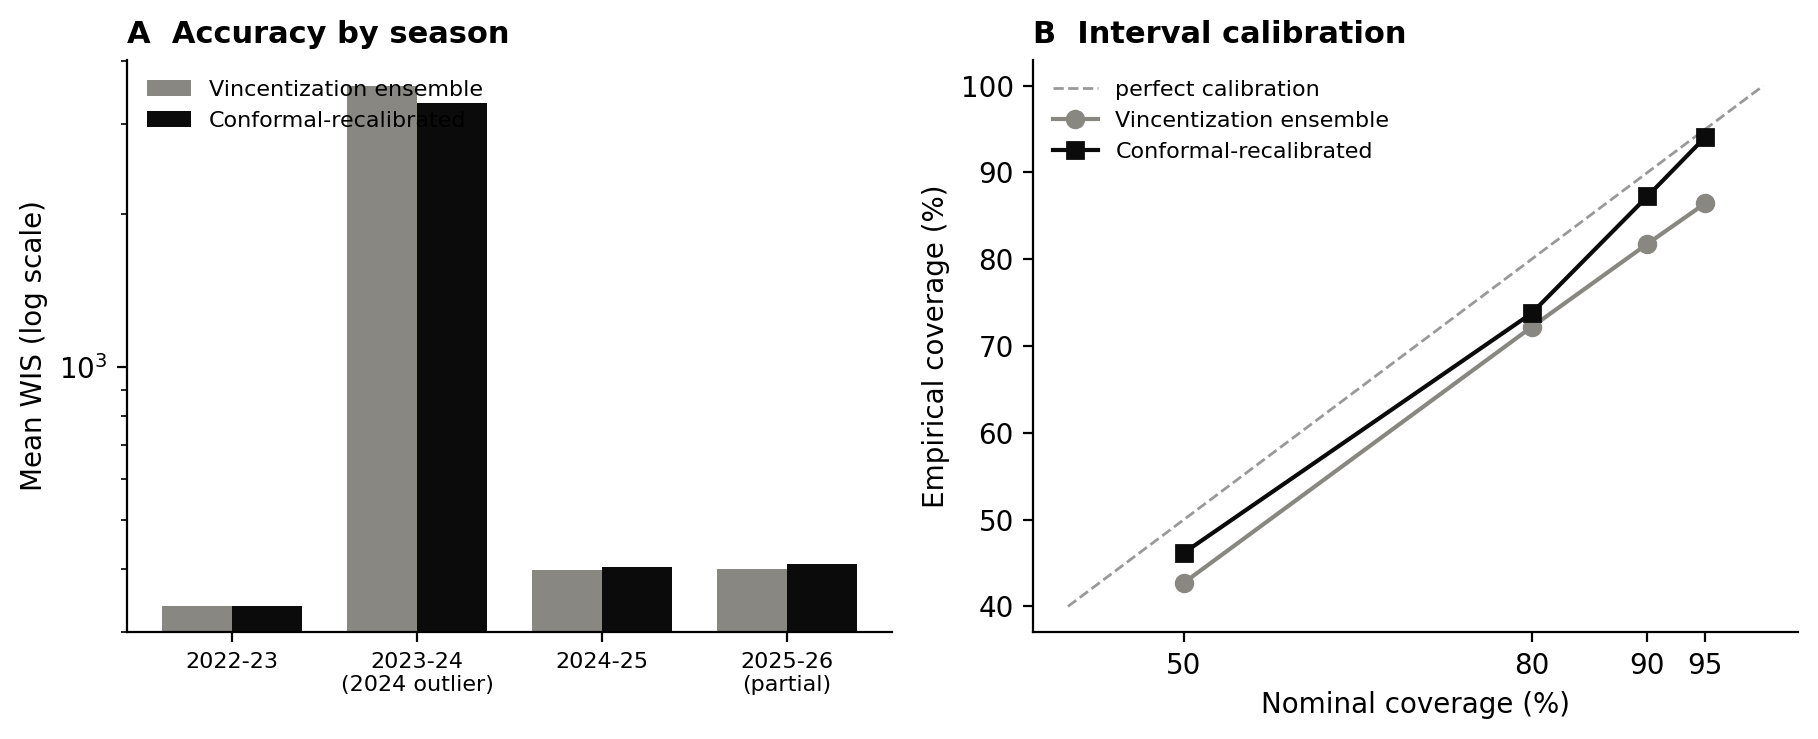
\includegraphics[width=0.92\textwidth]{../results/figures/paper_conformal.png}
\caption{\textbf{Effect of conformal recalibration on the dengue ensemble.} (A) Mean WIS by season,
Vincentization ensemble versus the conformal-recalibrated ensemble (log scale). The gain
concentrates in the 2024 outlier season at a small cost in ordinary seasons. (B) Interval
calibration: empirical versus nominal coverage. Recalibration moves the outer intervals (90, 95)
toward the diagonal.}
\label{fig:conformal}
\end{figure}

\subsection{The key differences are statistically significant}\label{sec:significance}
The absolute skill of each model carries wide uncertainty. A block bootstrap, repeatedly resampling
whole state-season units (with replacement) and recomputing normalized WIS on each resample to see
how much the result varies, over the 104
state-season units gives a 95 percent confidence interval (CI) on the conformal ensemble's
normalized WIS of
$[0.423, 0.639]$, and the intervals of the leading models overlap (Fig~\ref{fig:significance}A), a
direct consequence of the outbreak season inflating the variance of any magnitude-weighted score. The
comparisons that matter are nonetheless decisive, because the models are strongly correlated across
units, meaning they tend to do well or badly on the same state-seasons, so a paired analysis that
looks at each model's difference from another on the very same units cancels that shared,
season-driven variance instead of drowning in it (Fig~\ref{fig:significance}B).
The conformal recalibration improves on the median ensemble by a mean 71.3 WIS (95 percent CI
$[56.9, 87.8]$) and on the best single model, XGBoost, by 27.9 $([8.8, 47.3])$; on ordinary seasons
the deep network beats XGBoost by 48.9 $([14.9, 87.4])$; XGBoost itself beats the alternative
gradient-boosted implementation we also tested, LightGBM, by 111.1 $([81.6, 143.0])$; and the
conformal ensemble beats the naive
baseline by 395.1 $([338.8, 457.3])$. All five intervals exclude zero. The lesson is methodological as much
as substantive: in a record with one extreme season, marginal skill intervals are wide, but paired
comparisons remain informative and are the sound basis for model selection.

\begin{figure}[t]
\centering
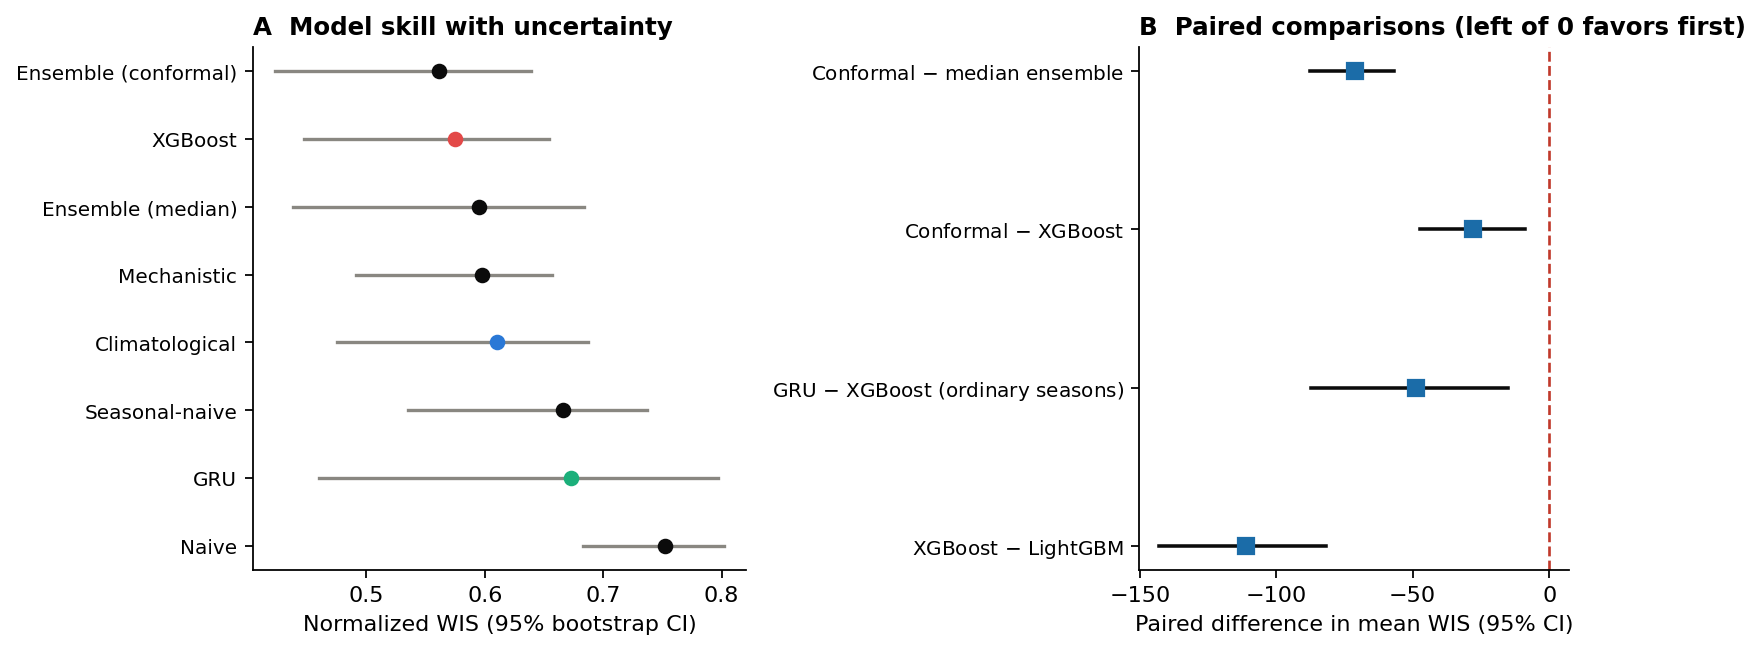
\includegraphics[width=0.95\textwidth]{../results/figures/paper_significance.png}
\caption{\textbf{Statistical significance of the model comparisons.} (A) Normalized WIS with 95
percent block-bootstrap intervals over state-season units; the leading models' intervals overlap
because the 2024 outbreak inflates the variance of absolute skill. (B) Paired differences in mean WIS
with 95 percent intervals; all four comparisons lie left of zero, so the conformal ensemble
significantly beats the median ensemble and XGBoost, the deep network significantly beats
XGBoost on ordinary seasons, and XGBoost significantly beats the alternative gradient-boosted
implementation we also tested, LightGBM.}
\label{fig:significance}
\end{figure}

\subsection{The winner depends on the evaluation metric}\label{sec:metric}
The overall mean WIS in Table~\ref{tab:leaderboard} is dominated by the largest states and by the
outbreak season, both of which contribute large absolute scores. The challenge's headline metric is
instead a normalized WIS, the sum of WIS divided by the sum of observed cases, which is scale-free
across regions. Under this metric the ordering changes in a revealing way. The conformal ensemble is
best over all folds (normalized WIS 0.561), consistent with the mean-WIS ranking. When the 2024
outlier is excluded to isolate ordinary-season skill, the deep network rises from worst of six
leading models by mean WIS to third-best by normalized WIS (0.385), and the plain median ensemble
overtakes the conformal ensemble for the single best spot on this metric (0.371 versus 0.375),
while the gradient-boosted model (XGBoost) falls from second-best to fifth of six (0.434) and the
mechanistic model falls from fourth to last (0.450) (Fig~\ref{fig:relwis}). The reversal is real but
milder for the gradient-boosted model than it was for the LightGBM configuration we tested first,
which fell all the way to the single weakest of the serious models under this metric (0.549, still
its value in Table~\ref{tab:leaderboard} since LightGBM itself was not adopted): XGBoost's more
balanced profile across seasons (Section~\ref{sec:noseason}) narrows, but does not eliminate, the
metric-dependent reordering that motivates reporting both metrics. The
disagreement is not a paradox. Consider two toy states, one with 10{,}000 weekly cases and one
with 100: a model that misses the large state's count by 1{,}000 and the small state's by 50 has a
much larger magnitude-weighted error, dominated by the 1{,}000, than a metric that instead scores
each state's error relative to its own size (a 10 percent miss on the large state versus a 50
percent miss on the small one, so a scale-free metric would actually rate the small state's
forecast as worse). A metric that rewards accuracy on a few very large states favors
different models than one that rewards accuracy on the many small states, and the 2024 season
inflates the mean for whichever model handles it least badly. We therefore report both magnitude-
and unit-weighted skill, and we caution that an epidemic-forecasting leaderboard reporting a single
aggregate can mislead. The cross-state skew has a clear geographic structure (Fig~\ref{fig:skillmap}):
forecast difficulty, measured by normalized WIS, is greatest in the dense, high-incidence southeastern
states and lowest in the low-incidence interior, so magnitude-weighted skill is determined by a few
states.

\begin{figure}[t]
\centering
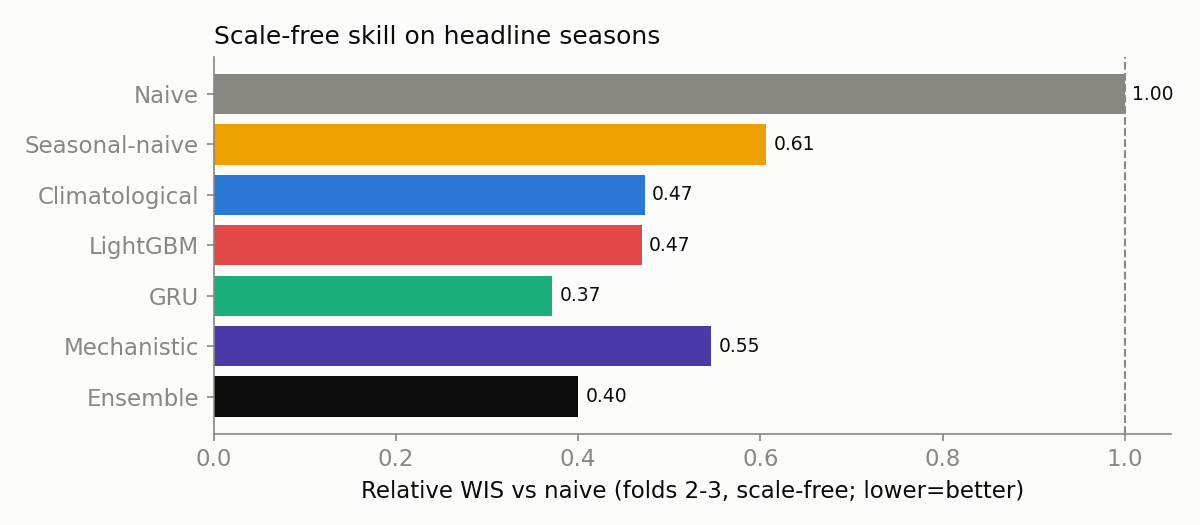
\includegraphics[width=0.72\textwidth]{../results/figures/paper_relative_wis.png}
\caption{\textbf{The best model depends on the metric.} Model rank by magnitude-weighted mean WIS
over all seasons (left) and by normalized WIS over the ordinary seasons with the 2024 outlier
excluded (right); rank 1 is best, among these six models. The rankings reorder: the deep network
rises from last by mean WIS to third on ordinary seasons, the gradient-boosted model (XGBoost) falls
from second to fifth, the mechanistic model falls from fourth to last, and the plain median ensemble
overtakes the conformal ensemble for the top spot. Values in parentheses are mean WIS (left) and
normalized WIS (right).}
\label{fig:relwis}
\end{figure}

\begin{figure}[t]
\centering
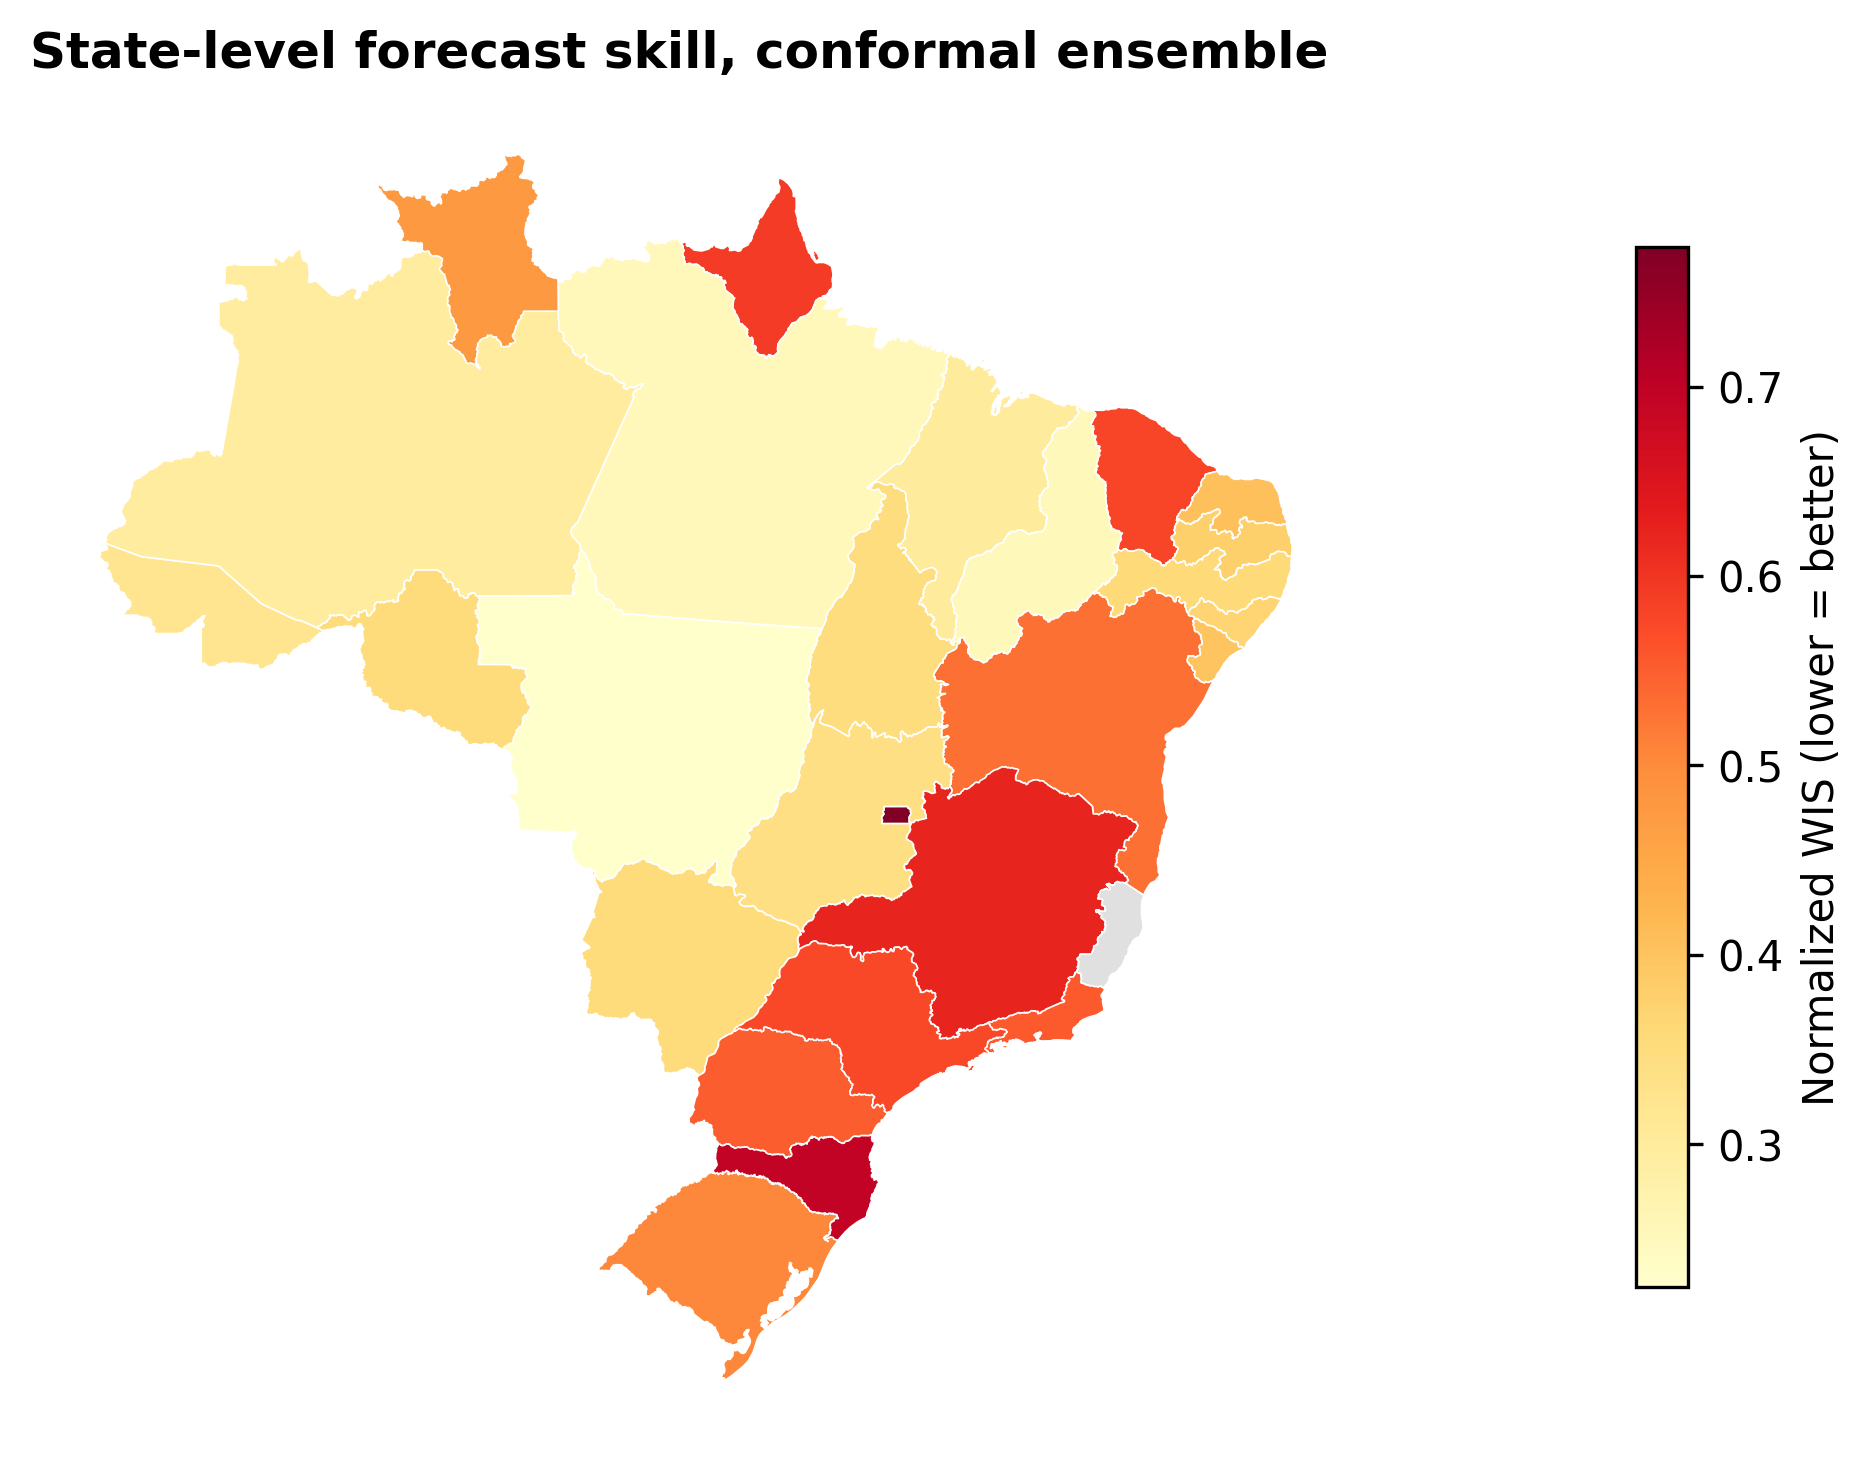
\includegraphics[width=0.72\textwidth]{../results/figures/paper_skill_map.png}
\caption{\textbf{Geographic structure of forecast skill.} Normalized WIS of the conformal ensemble by
state (lower is better). Forecasting is hardest in the dense, high-incidence southeastern states and
in the Federal District, and easiest in the low-incidence interior, which is why magnitude-weighted
skill is dominated by a few states. Espírito Santo (grey) is excluded from the challenge.}
\label{fig:skillmap}
\end{figure}

\subsection{Calibration and its correction}\label{sec:calibration}
Raw gradient-boosted and deep-learning quantile models are over-confident
(Fig~\ref{fig:coverage}): their nominal coverage, the fraction of outcomes an interval is supposed
to contain, e.g. 90 percent for the 90 percent interval, is higher than their empirical coverage,
the fraction it actually does contain. The GRU's nominal 50 percent
interval only actually contains the truth 27 percent of the time, and its nominal 95 percent
interval only 67 percent of the time, and it is under-covered in every season
rather than only in the outbreak year, which identifies the problem as systematic overconfidence
rather than a regime-specific failure. Conformalized quantile regression restores the gradient-boosted
model (XGBoost) to near-nominal calibration (48/79/88/92) at negligible WIS cost. The same correction applied
to the deep network trades away sharpness, how narrow and therefore informative its intervals are,
on the seasons where it is already accurate, so
calibration and sharpness trade off at the level of a single model. The per-quantile median of the
ensemble provides a structural calibration improvement at no cost, and the conformal recalibration
of Section~\ref{sec:conformal} completes it.

\begin{figure}[t]
\centering
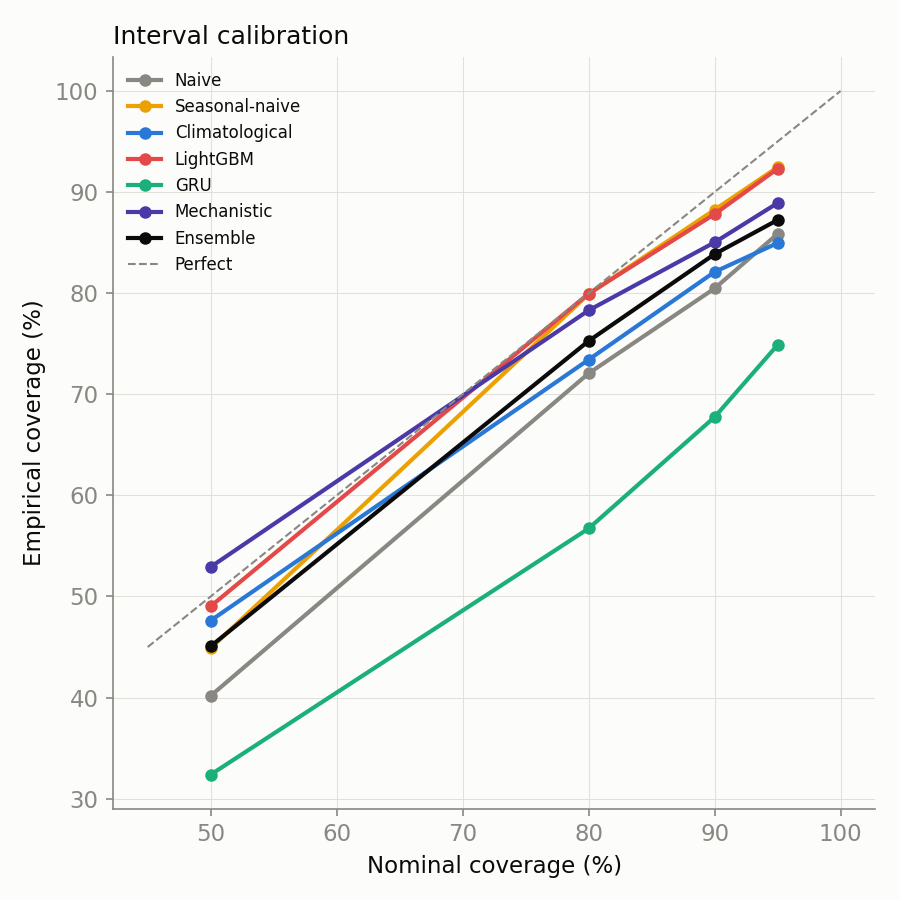
\includegraphics[width=0.6\textwidth]{../results/figures/paper_coverage.png}
\caption{\textbf{Interval calibration by model.} Empirical versus nominal coverage; points on the
diagonal are perfectly calibrated. The deep network is markedly overconfident; conformalized
quantile regression corrects the gradient-boosted model, and the conformal-recalibrated ensemble
tracks the diagonal at the outer intervals.}
\label{fig:coverage}
\end{figure}

\subsection{Skill varies with horizon, and the outbreak failure is under-prediction}\label{sec:robustness}
Because the 15-week reporting gap places every target 16 to 67 weeks ahead, we stratified skill by
lead time on the ordinary seasons (Fig~\ref{fig:robustness}A). The deep network's advantage is
horizon-dependent: it is the best model at short lead times (normalized WIS 0.255 at 16 to 27 weeks)
but degrades at the longest horizons (0.388 at 52 to 67 weeks), where both the conformal ensemble
(0.338) and the gradient-boosted model (0.349) overtake it. The conformal ensemble is the most
stable model across horizons and is never
worst, which mirrors its stability across seasons. WIS decomposes exactly into three non-negative
components (Section~\ref{sec:methods-scoring}): dispersion (a penalty for interval width, present
even when the forecast is centered correctly), under-prediction, and over-prediction; decomposing it
this way explains the
outbreak-season failure directly (Fig~\ref{fig:robustness}B): in the 2024 season the ensemble's score
is dominated by under-prediction (a mean of 2675 WIS units, against 621 for dispersion and 1 for
over-prediction), whereas every other season is dominated by dispersion, i.e. is driven by ordinary
interval width rather than the forecast being systematically off in either direction. The record epidemic was not
mis-shaped but simply larger than any model would predict from pre-season information, which is why
widening the upper tail, as the conformal recalibration does, is the effective remedy.

\begin{figure}[t]
\centering
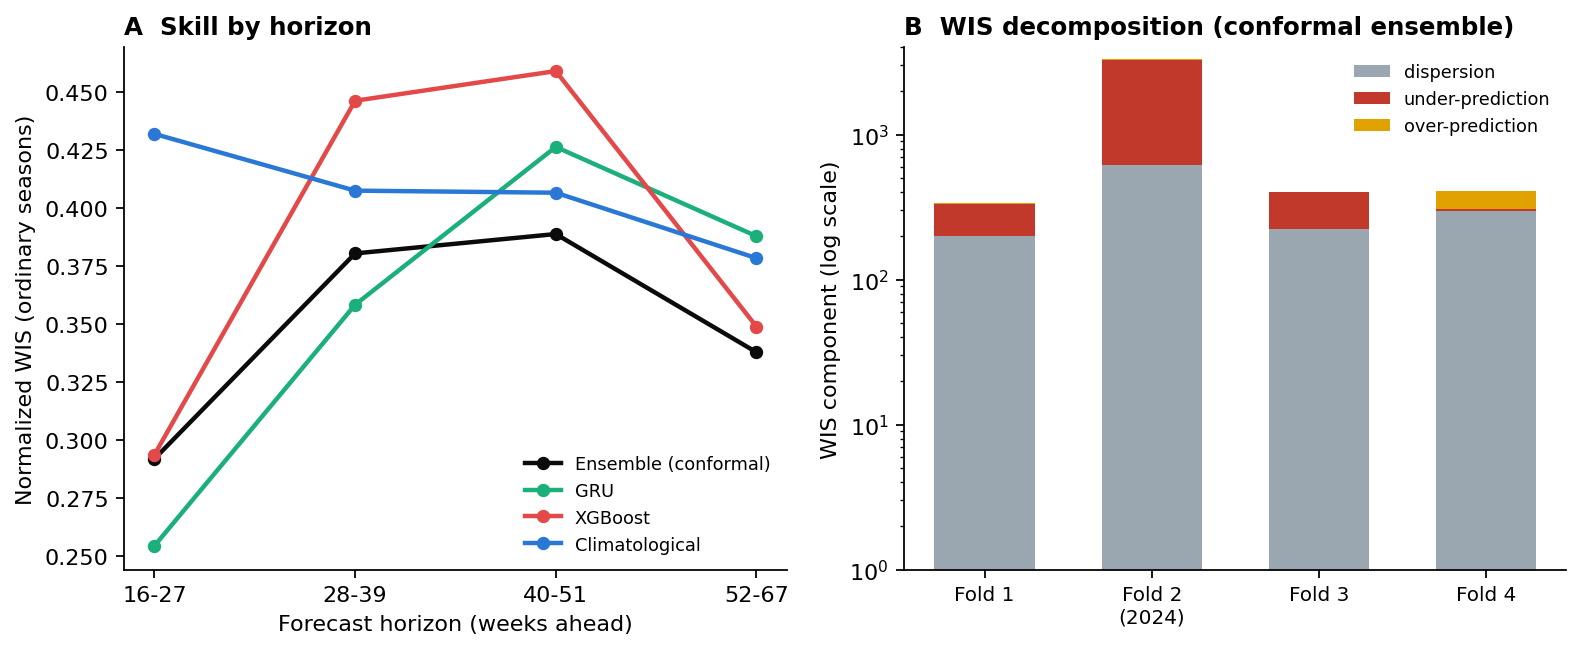
\includegraphics[width=0.95\textwidth]{../results/figures/paper_robustness.png}
\caption{\textbf{Robustness across horizons and anatomy of the outbreak-season failure.} (A)
Normalized WIS by forecast horizon on the ordinary seasons; the deep network leads at short lead times
and fades at long ones, while the conformal ensemble is stable. (B) WIS decomposition of the conformal
ensemble by season (log scale); the 2024 season is dominated by under-prediction, not by dispersion or
over-prediction.}
\label{fig:robustness}
\end{figure}

\subsection{Added complexity did not improve forecasts}\label{sec:negative}
Four interventions that plausibly should have helped did not (Table~\ref{tab:ablation}). First,
adding observed-climate covariates to the gradient-boosted model, following the distributed-lag
non-linear (DLNM) structure of the strongest model in the 2024 sprint, which lets a covariate's
effect on cases be both delayed (this week's temperature can affect cases several weeks later, not
just this week) and non-linear \citep{araujo2026,gasparrini2010},
worsened backtest WIS by 3.3 percent (1299 to 1342 on the LightGBM configuration on which this test
was originally run\footnote{This test and the hyperparameter-tuning test below were originally
performed on the LightGBM-based pipeline before it was superseded by XGBoost
(Section~\ref{sec:methods}) and before a later data refresh. Re-verified on the current
XGBoost-based pipeline and current data (2026-09-09): the climate-covariate finding replicates in
the same direction (WIS 1166 $\rightarrow$ 1190 without vs.\ with the covariates, a 2.0 percent
degradation from adding them, versus the original 3.3 percent). The hyperparameter-tuning finding
does \emph{not} replicate: on XGBoost, the config an internal fold-1 holdout preferred (shallower
trees, \texttt{max\_depth} 3 vs.\ the deployed default 5, with stronger leaf-size regularization)
also won the true 4-fold backtest on every single fold (WIS 1190 $\rightarrow$ 1152, a genuine 3.2
percent improvement, not an overfit to the holdout) -- the opposite of the LightGBM-era finding
described in the main text below. We report both results rather than silently replacing the
original figures, since the discrepancy is itself informative: whether an internal-holdout
hyperparameter search transfers to the true backtest evidently depends on the specific model
family and hyperparameter space searched, not a fixed property of this forecasting task. This
XGBoost re-verification was checked at the ensemble level under this project's own fold-1 tuning
discipline (the same check used to validate the original LightGBM-to-XGBoost swap) and did
\emph{not} pass: combined with climatological\_quantile and gru\_negbin and conformal-recalibrated,
both the shallower-hyperparameter config alone and combined with dropping the climate covariates
lose on fold 1 (WIS 347 and 346 respectively, vs.\ the deployed ensemble's 337) despite winning on
every full-aggregate metric -- the same overfitting-to-the-reporting-folds pattern this project has
already caught in other candidate changes (Section~\ref{sec:negative}). Dropping the climate
covariates alone does pass fold 1 at the ensemble level (335 vs.\ 337) but is a mixed result
elsewhere (worse raw WIS and normalized WIS all-folds, better normalized WIS excluding 2024) rather
than a clean sweep. None of the three candidates were adopted; the deployed ensemble is unchanged.}).
A feature-importance
analysis showed why: the nine
added covariates (minimum temperature, a derived standardized-precipitation drought index at one,
three, and six month accumulations, multi-month temperature lags, thermal range, and rainy days)
together carried only 5.3 percent of importance and ranked below the existing features. The climate
signal the model actually uses is the seasonal climate forecast and the El Ni\~no--Southern
Oscillation indices, both already present and both forward-looking, rather than observed local
weather, which is stale at the long horizons that dominate a full-season forecast. Second, a
hierarchical, empirical-Bayes pooling of each state's seasonal climatology toward its macroregion,
that is, borrowing statistical strength by pulling each state's estimate partway toward its
region's average rather than trusting each state's own history entirely,
worsened the ensemble from 1162 to 1185, because Brazilian states are too heterogeneous within a
macroregion: shrinking a small state toward a region dominated by a larger, differently behaving
state introduces bias. Third, a hyperparameter search that improved an internal time-block holdout,
a held-out slice of recent training weeks used to tune hyperparameters before touching the real
backtest,
by 5 percent worsened the true backtest on the LightGBM configuration this was originally tested
on, because an internal holdout does not necessarily represent forecasting a full future season
from mid-year; conservative, a priori defaults generalized better in that specific test. A
re-verification on the current XGBoost-based pipeline found the opposite as a standalone model (see
footnote above): the holdout's preferred configuration also won the true backtest there. Checked
further at the ensemble level, though, it lost on the same fold-1 tuning check that validated every
other change reported here, so it was not adopted -- a reminder that a standalone-model result and
an ensemble-level result can disagree even when both are individually rigorous. Fourth, we tested the ensemble combination
rule itself: the inaugural 2024 sprint's organizers combine models by log-linear (logarithmic)
pooling of parametric predictive distributions \citep{araujo2026,carvalho2023}, a genuinely
different rule from our per-quantile-median Vincentization -- a precision-weighted combination of
distributions rather than a per-quantile order statistic, which guarantees a unimodal result.
Substituted for Vincentization (equal weights, then conformal-recalibrated identically to the
deployed ensemble), it wins three of four folds outright, including fold 1, the only fold this
project's discipline permits for tuning decisions (WIS 309 versus 337, an 8 percent improvement)
and the ordinary-season metric (normalized WIS excluding 2024, 0.338 versus 0.375). By the letter
of that discipline, this candidate passes and every previous one in this table failed. But it loses
specifically on the 2024 outbreak fold (WIS 3630 versus 3297, a 10 percent regression, with 90 and
95 percent coverage both falling further from nominal, 64/79 versus 70/83): precision-weighted
pooling is sharper in ordinary seasons but narrows the combined tails exactly where the widest
tails matter most. We did not adopt it. The fold-1 rule exists to prevent tuning the ensemble to
the specific reporting folds it is judged on, not to license a change that measurably weakens
performance on the one season the entire ensemble-plus-conformal design is built to protect
against; a rule applied mechanically here would have recommended trading away the outbreak-season
robustness that motivates this paper's central design choice. Together these
results locate much of the predictable signal in this problem, caution against complexity that is
not validated on the true forecasting task, and show that even a validation discipline's own
conclusions can be implementation-specific -- and occasionally require judgment beyond the rule
itself -- rather than a fixed property of the problem.

\begin{table}[t]
\centering\small
\caption{\textbf{Interventions that did not help, plus two that passed part of our validation
discipline but still were not adopted (negative results throughout).} Each was evaluated on
the same backtest as the main comparison. $^{\dagger}$Originally tested on the LightGBM
configuration before it was superseded by XGBoost and before a later data refresh; re-verified on
the current XGBoost-based pipeline and current data (see footnote in text). The hyperparameter
row's standalone-model finding reversed on re-verification, but checking it at the ensemble level
(the same fold-1 discipline that validated every adopted change) found it should not be adopted
either. $^{\ddagger}$Passes the fold-1 tuning check outright but regresses specifically on the
outbreak fold (see text); not adopted on substantive grounds despite passing the formal rule --
none of these five rows changed the deployed model.}
\label{tab:ablation}
\begin{tabular}{@{}lll@{}}
\toprule
\textbf{Intervention} & \textbf{Effect} & \textbf{Reason} \\
\midrule
Observed-climate covariates$^{\dagger}$ & WIS 1166 $\rightarrow$ 1190 (current); & 5.3\% importance; signal is \\
 (XGBoost) & 1299 $\rightarrow$ 1342 (orig.) & forecast + ENSO, not observed weather \\
Hierarchical macroregion pooling & WIS 1162 $\rightarrow$ 1185 & small-state bias; too correlated \\
 (added to ensemble) & & with climatological member \\
Hyperparameter tuning$^{\dagger}$ & internal holdout $+5\%$, & internal holdout misrepresented \\
 (LightGBM, original) & backtest worse & full-season forecasting \\
Hyperparameter tuning$^{\dagger}$ & standalone $-3.2\%$; & generalized alone, but not \\
 (XGBoost) & ensemble fold 1 worse & at ensemble level (see text) \\
Log-linear pooling$^{\ddagger}$ & fold 1 $-8\%$; outbreak fold & sharper pooling narrows tails \\
 (vs.\ Vincentization) & (fold 2) WIS $+10\%$ & exactly where width matters most \\
\bottomrule
\end{tabular}
\end{table}

\subsection{Chikungunya is a more predictable, contrasting target}\label{sec:chik}
Brazil reported roughly 422{,}000 chikungunya cases in 2024, a cumulative incidence near 199 per
100{,}000, and the virus has recurred across the country since its 2014 introduction with a spatial
pattern shaped by heterogeneous population immunity~\citep{desouza2023}.
We forecast chikungunya on the same 26 states, harness, and seasons as dengue. Two differences stand
out. First, the gradient-boosted model alone is the best forecaster (WIS 79.1), ahead of the ensemble
(89.5) and every other model (Table~\ref{tab:chik}); it is best in every season
(Table~\ref{tab:chikfold}), so combining it with weaker models only dilutes it. Second, chikungunya is
markedly more predictable than dengue relative to its scale: the 2024 season is only modestly harder
than the others (mean WIS 120 versus a range of 33 to 81 across seasons), in contrast to the
order-of-magnitude jump dengue shows in 2024. This matches reports that chikungunya dynamics in Brazil
are more regular than dengue's~\citep{desouza2023}, plausibly because immunity accumulates
against a single antigenic type rather than interacting across four co-circulating dengue serotypes.
The practical consequence is that the best model is disease-specific: a blended ensemble is right for
dengue, a single well-calibrated learner for chikungunya, even within one surveillance system and
pipeline.

\begin{table}[t]
\centering\small
\caption{\textbf{Chikungunya backtest.} State-level, same harness and seasons as dengue. Gradient
boosting alone is best.}
\label{tab:chik}
\begin{tabular}{@{}lrcc@{}}
\toprule
\textbf{Model} & \textbf{WIS} & \textbf{Cov.\ 50 (\%)} & \textbf{Cov.\ 90 (\%)} \\
\midrule
LightGBM                  & \textbf{79.1} & 47 & 88 \\
Ensemble (Vincentization) & 89.5 & 55 & 87 \\
Climatological            & 92.4 & 56 & 85 \\
Seasonal-naive            & 95.1 & 48 & 88 \\
Mechanistic               & 99.5 & 53 & 86 \\
Naive                     & 119.1 & 41 & 80 \\
\bottomrule
\end{tabular}
\end{table}

\begin{table}[t]
\centering\small
\caption{\textbf{Chikungunya mean WIS by season.} LightGBM is best in every season, unlike dengue, and
the 2024 season (fold 2) is only modestly harder than the others.}
\label{tab:chikfold}
\begin{tabular}{@{}lrrrr@{}}
\toprule
\textbf{Model} & \textbf{Fold 1} & \textbf{Fold 2} & \textbf{Fold 3} & \textbf{Fold 4} \\
\midrule
LightGBM                  & \textbf{81.2} & \textbf{120.2} & \textbf{69.2} & \textbf{33.4} \\
Ensemble (Vincentization) & 88.7 & 141.1 & 73.8 & 41.5 \\
Climatological            & 94.3 & 143.3 & 75.3 & 43.7 \\
Seasonal-naive            & 92.8 & 152.3 & 77.1 & 44.6 \\
Mechanistic               & 92.1 & 166.6 & 77.0 & 48.6 \\
Naive                     & 181.3 & 145.7 & 75.3 & 57.7 \\
\bottomrule
\end{tabular}
\end{table}

\subsection{City-level forecasting is substantially harder}\label{sec:city}
The challenge also solicits municipal forecasts for 15 dengue and 10 chikungunya cities, an optional
target we submitted with the climatological quantile model. City-level forecasting is much harder than
state-level: the best model's normalized WIS is 0.60 for dengue cities and 0.87 for chikungunya cities
(Table~\ref{tab:city}), against 0.56 and 0.62 at the state level. Interval coverage is also poorer (50
percent coverage of 39 percent for dengue cities), because many mid-sized municipalities have episodic,
over-dispersed series with long runs of zero counts that a per-week empirical quantile under-covers. A
degenerate all-zero median is a concrete failure mode of these sparse series, which we addressed by
switching the point forecast to a clamped predictive mean, the distribution's mean rather than its
median, floored at zero so it can never predict a negative case count; a principled zero-inflated
treatment is a
clear direction for the municipal tracks. These results quantify the resolution penalty of forecasting
at the level where interventions are delivered.

\begin{table}[t]
\centering\small
\caption{\textbf{City-level backtest} (optional tracks; climatological quantile model submitted). WIS
and normalized WIS averaged over the target cities and four seasons. For chikungunya cities,
climatological and seasonal-naive are statistically indistinguishable (WIS 30.17 versus 30.17); no
value is bolded there for that reason.}
\label{tab:city}
\begin{tabular}{@{}llrrc@{}}
\toprule
\textbf{Disease} & \textbf{Model} & \textbf{WIS} & \textbf{nWIS} & \textbf{Cov.\ 50 (\%)} \\
\midrule
Dengue (15 cities)      & Climatological & \textbf{123.3} & \textbf{0.60} & 39 \\
                        & Seasonal-naive & 131.8 & 0.64 & 30 \\
                        & Naive          & 133.5 & 0.65 & 30 \\
\addlinespace
Chikungunya (10 cities) & Climatological & 30.2 & 0.87 & 57 \\
                        & Seasonal-naive & 30.2 & 0.87 & 50 \\
                        & Naive          & 34.4 & 1.00 & 33 \\
\bottomrule
\end{tabular}
\end{table}

\subsection{Onset, peak, and total burden are decision-relevant summaries that WIS does not
directly show}\label{sec:operational}
WIS scores every week of the season equally, but health-system planning asks three narrower
questions: when will the season start, how large will the peak be, and how many cases will there
be in total. We compute, per state-season unit, the error in the first week each series reaches 10
percent of its own peak (onset), the timing and log-magnitude error at the true peak week (as in
Section~\ref{sec:noseason}), and the log-ratio of predicted to observed total season cases
(Table~\ref{tab:operational}). No model wins on every one of these summaries, which is the same
qualitative pattern as the main WIS results but on a different, more directly interpretable set of
outputs. The gradient-boosted model (XGBoost) has the lowest onset-timing error (3.7 weeks mean
absolute
error, against 3.8 for the conformal ensemble), the climatological model has the lowest peak-timing
error (4.5 weeks, against 4.9 for the ensemble), and the gradient-boosted model again gives the
least biased total-season case count (a log-ratio of $-0.01$, i.e. predicting within 1 percent of
the true total at the median unit, against 20
percent under-prediction for the ensemble and 56 percent for the mechanistic model). Every model under-predicts case
counts at the true peak week specifically, by 42 to 76 percent at the median unit, more than it
under-predicts the season total, which shows that the harder part of the forecasting problem is
capturing acute intensity at the peak rather than accumulated burden over the season. The ensemble
is a reasonable middle choice on every one of these summaries without being the best on any single
one, consistent with it being chosen for robustness (Section~\ref{sec:noseason}) rather than for
leading any one metric.

\begin{table}[t]
\centering\small
\caption{\textbf{Onset, peak, and total-burden accuracy}, dengue state-level, four seasons and 26
states (104 units). Onset and peak-week errors are mean absolute error in weeks. Peak magnitude and
total cases are the median log(predicted / observed) at the true peak week and over the full season
respectively; 0 is unbiased, negative is under-prediction. Best value in each column is in bold.}
\label{tab:operational}
\begin{tabular}{@{}lrrrr@{}}
\toprule
\textbf{Model} & \textbf{Onset MAE} & \textbf{Peak-week MAE} & \textbf{Peak magnitude} & \textbf{Total cases} \\
 & (weeks) & (weeks) & (log-ratio) & (log-ratio) \\
\midrule
Ensemble (conformal)   & 3.8 & 4.9 & $-0.71$ & $-0.22$ \\
XGBoost                & \textbf{3.7} & 5.3 & \textbf{$-0.55$} & \textbf{$-0.01$} \\
Climatological         & 4.2 & \textbf{4.5} & $-0.85$ & $-0.32$ \\
GRU (deep learning)    & 4.1 & 5.0 & $-0.59$ & $-0.12$ \\
Mechanistic            & 4.1 & 5.0 & $-1.43$ & $-0.83$ \\
Seasonal-naive         & 4.2 & 4.8 & $-0.82$ & $-0.30$ \\
Naive                  & 4.9 & 17.4 & $-1.13$ & $-0.14$ \\
\bottomrule
\end{tabular}

\smallskip
\footnotesize Naive is the worst model by every measure in this table, including a 17-week
peak-timing error; unlike in an earlier data vintage of this analysis, its total-cases figure no
longer happens to look artificially competitive, which is itself a reminder that a single
season-total number, like a single aggregate WIS, can be sensitive to incidental error cancellation
and should not be read in isolation from the other columns.
\end{table}

\section{Discussion}

\subsection{Robustness under regime shift}
The most consequential finding is that model rankings are season-dependent and can invert in an
outbreak year. A model chosen for its average score can be the least reliable in the season for which
forecasts matter most, as the deep network is here. Two responses follow. One is to combine models,
so that no single failure mode determines the forecast; the ensemble is never worst in any season
and is best overall once recalibrated. The other is to prefer models whose uncertainty widens under
distribution shift, as the mechanistic model's bootstrap-of-historical-seasons intervals do. These
observations align with evidence from collaborative forecast hubs, where combined forecasts are
consistently competitive with or better than their members \citep{cramer2022,reich2019,sherratt2023}.

\subsection{Metric choice is a reporting-standards issue}
The identity of the best model changes with the aggregation of skill across a highly skewed set of
states. This is not specific to our models or to Brazil. Any national forecasting evaluation with
strong heterogeneity in population and incidence faces the same tension between magnitude-weighted
and unit-weighted skill. Reporting a single aggregate obscures it. We recommend reporting both, as
the interval-score and forecast-hub literature increasingly does \citep{bracher2021}, and we treat
the normalized WIS the challenge adopts as the headline while retaining magnitude-weighted mean WIS
and per-unit relative WIS alongside it.

\subsection{Simple methods and the limits of complexity}
Deep learning did not dominate, and simple methods, a climatological quantile model and a bootstrap
of historical seasons, were hard to beat. This is consistent with forecasting-competition evidence
that in small-sample, few-series regimes, parsimonious methods and combinations are strong
\citep{makridakis2020}. The pattern recurs one sprint earlier: in IMDC24, a Bayesian baseline model
using no climate covariates at all was among the most consistently competitive submissions across
states and seasons \citep{araujo2026}, echoing our own finding that a covariate-free climatological
baseline and a historical-trajectory bootstrap are hard to beat with more heavily engineered
alternatives. The same predecessor sprint offers an independent caution about tuning ensembles on
limited past data: its CRPS-weighted logarithmic-pooling ensemble, with weights fit to 2023--2024
performance, badly overestimated the true 2025 outbreak in three of five states, because the
models it weighted most heavily had performed well on those past seasons but poorly on the actual
target season \citep{araujo2026} -- the same overfitting-to-past-folds failure mode our fold-1
tuning discipline (Section~\ref{sec:negative}) exists to catch, now observed independently in
another team's ensemble on a different edition of the same challenge. Our negative results sharpen
the point. The covariate that helped the
strongest 2024-sprint model, climate acting through a distributed-lag non-linear response
(DLNM, Section~\ref{sec:negative} above) \citep{lowe2021,gasparrini2010}, did not help our gradient-boosted forecaster, because that
structure requires the regularized, partially pooled Bayesian formulation in which it was developed,
whereas an unregularized tree over the same inputs overfits low-signal dimensions. The forecast-relevant
climate information in our pipeline is the seasonal forecast and large-scale oscillation indices, not
observed local weather. This clarifies where future modeling effort should go: toward a Bayesian
spatiotemporal member that can use climate through an exposure-lag-response surface, rather than
toward more covariates in a boosted model.

\subsection{Conformal recalibration as transferable insurance}
The conformal recalibration is simple, scale-free, and cheap, and it improves both accuracy and
calibration. It connects to conformalized quantile regression \citep{romano2019} and to the broader
literature on adaptive conformal methods for distribution shift \citep{gibbs2021,zaffran2022}, which
similarly recalibrate intervals in response to a changing data-generating process rather than
assuming a fixed noise scale, though those methods update continuously as new data arrive whereas
ours is calibrated once, on a single tuning season. Because it widens mainly the outer
tails, it protects against the failure mode that dominates the outbreak season without materially
degrading ordinary-season sharpness. For an operational forecaster who cannot know in advance whether
the coming season will be ordinary or extreme, this asymmetric protection is the right default.

\subsection{Limitations}
The fourth backtest season is only partially resolved in the available data and is reported
separately; its numbers will firm up as the 2025--26 season completes. Municipality-to-state
aggregation discards sub-state epidemic asynchrony that a municipal model could exploit. The study
covers two diseases in one country and is retrospective; we submitted the recalibrated ensemble to
the challenge's forecast phase (the true 2026--27 season, EW41 2026 through EW40 2027) ahead of its
2026-09-10 deadline, but a genuine prospective score awaits that season's resolution. The comparison
is single-team, so it does not capture the full diversity
of approaches a multi-team sprint would, though our 26-state, four-track design covers more
geographic and epidemiological ground than the inaugural 2024 sprint, which evaluated five highly
endemic states and explicitly left lower-incidence, more recently affected regions untested
\citep{araujo2026}; the conformal factors are calibrated on one season under
the challenge's tuning-fold discipline rather than by a fully online procedure. Finally, the
2023--24 outlier season we treat as a pure epidemiological surge may also reflect a data-quality
confound: the 2024 season saw a substantial expansion of Oropouche fever, whose symptoms overlap
with dengue's, and the inaugural sprint's organizers flag possible dengue-notification
contamination from Oropouche misclassification as a contributing factor to that season's models
failing so widely \citep{araujo2026}, a possibility our own pipeline cannot rule out with
notification data alone.

\subsection{Future work}
The immediate next step is scoring the submitted forecast phase once the 2026--27 season resolves,
which will provide a genuine prospective test of the recalibrated ensemble. Beyond it, four
directions follow from our results and from the challenge organizers' own stated plans. First, a
Bayesian spatiotemporal or endemic-epidemic member with a distributed-lag non-linear climate
response \citep{held2005,meyer2017}, which our negative result suggests is the right home for
climate covariates. Second, hierarchical reconciliation across state, city, and national forecasts
for coherence. Third, municipal-level feature engineering for the optional city tracks. Fourth, the
organizers report moving their own collective ensemble toward a copula-based approach that samples
coherent full-trajectory epidemic curves rather than combining marginal per-week quantiles
independently; our per-quantile median ensemble does not guarantee this, but our mechanistic
model's bootstrap of complete historical trajectories already provides trajectory-level coherence by
construction, which is a reason to prefer it, or a copula-linked resampling of it, over a purely
per-week combination when coherent full-season trajectories rather than marginal weekly intervals
are the target.

\section{Materials and methods}\label{sec:methods}

\subsection{Pipeline overview}\label{sec:pipeline-overview}
Fig~\ref{fig:pipeline} summarizes the full pipeline end to end before the following subsections
detail each stage. Raw weekly surveillance and covariate data (Section~\ref{sec:methods-data}, below)
are filtered to each fold's own training cutoff, which removes any observation dated after that
cutoff before anything downstream can see it (Section~\ref{sec:methods-backtest}). For the machine-learning
families, the cutoff-filtered history is expanded into a synthetic-origin training panel: every
historical week becomes a candidate forecast origin, paired with the realized value at horizons 1
to 67 weeks ahead, which supplies enough training examples for gradient boosting and the deep
network despite only four official evaluation windows existing. Four model families are then fit
independently per fold: baselines and the climatological quantile model, a gradient-boosted model
with conformalized
quantile regression, the GRU deep ensemble, and the semi-mechanistic trajectory bootstrap. We
evaluated two gradient-boosting implementations on the identical panel, LightGBM \citep{ke2017} and
XGBoost \citep{chen2016}, and adopted XGBoost, which scored significantly better
(Section~\ref{sec:significance}; Fig~\ref{fig:significance}). The
climatological, XGBoost, and GRU outputs (not the mechanistic model, which is evaluated separately
for comparison) are combined by per-quantile median (Vincentization) into an ensemble, which is then
conformally recalibrated using widening factors estimated once on a designated tuning season
(Section~\ref{sec:methods-conformal}). The output at every stage is the same canonical shape, nine
quantiles per state or city and week, and the final recalibrated quantiles are validated against the
platform's submission schema (non-negative, correctly nested, no date gaps) before being written out.
Chikungunya-state and the two optional city tracks follow the same pipeline but submit a single
family's output directly (LightGBM for chikungunya-state, unchanged from the dengue pipeline's
original configuration, climatological for both city tracks; see
Sections~\ref{sec:chik} and \ref{sec:city}) rather than the three-member ensemble.

\begin{figure}[t]
\centering
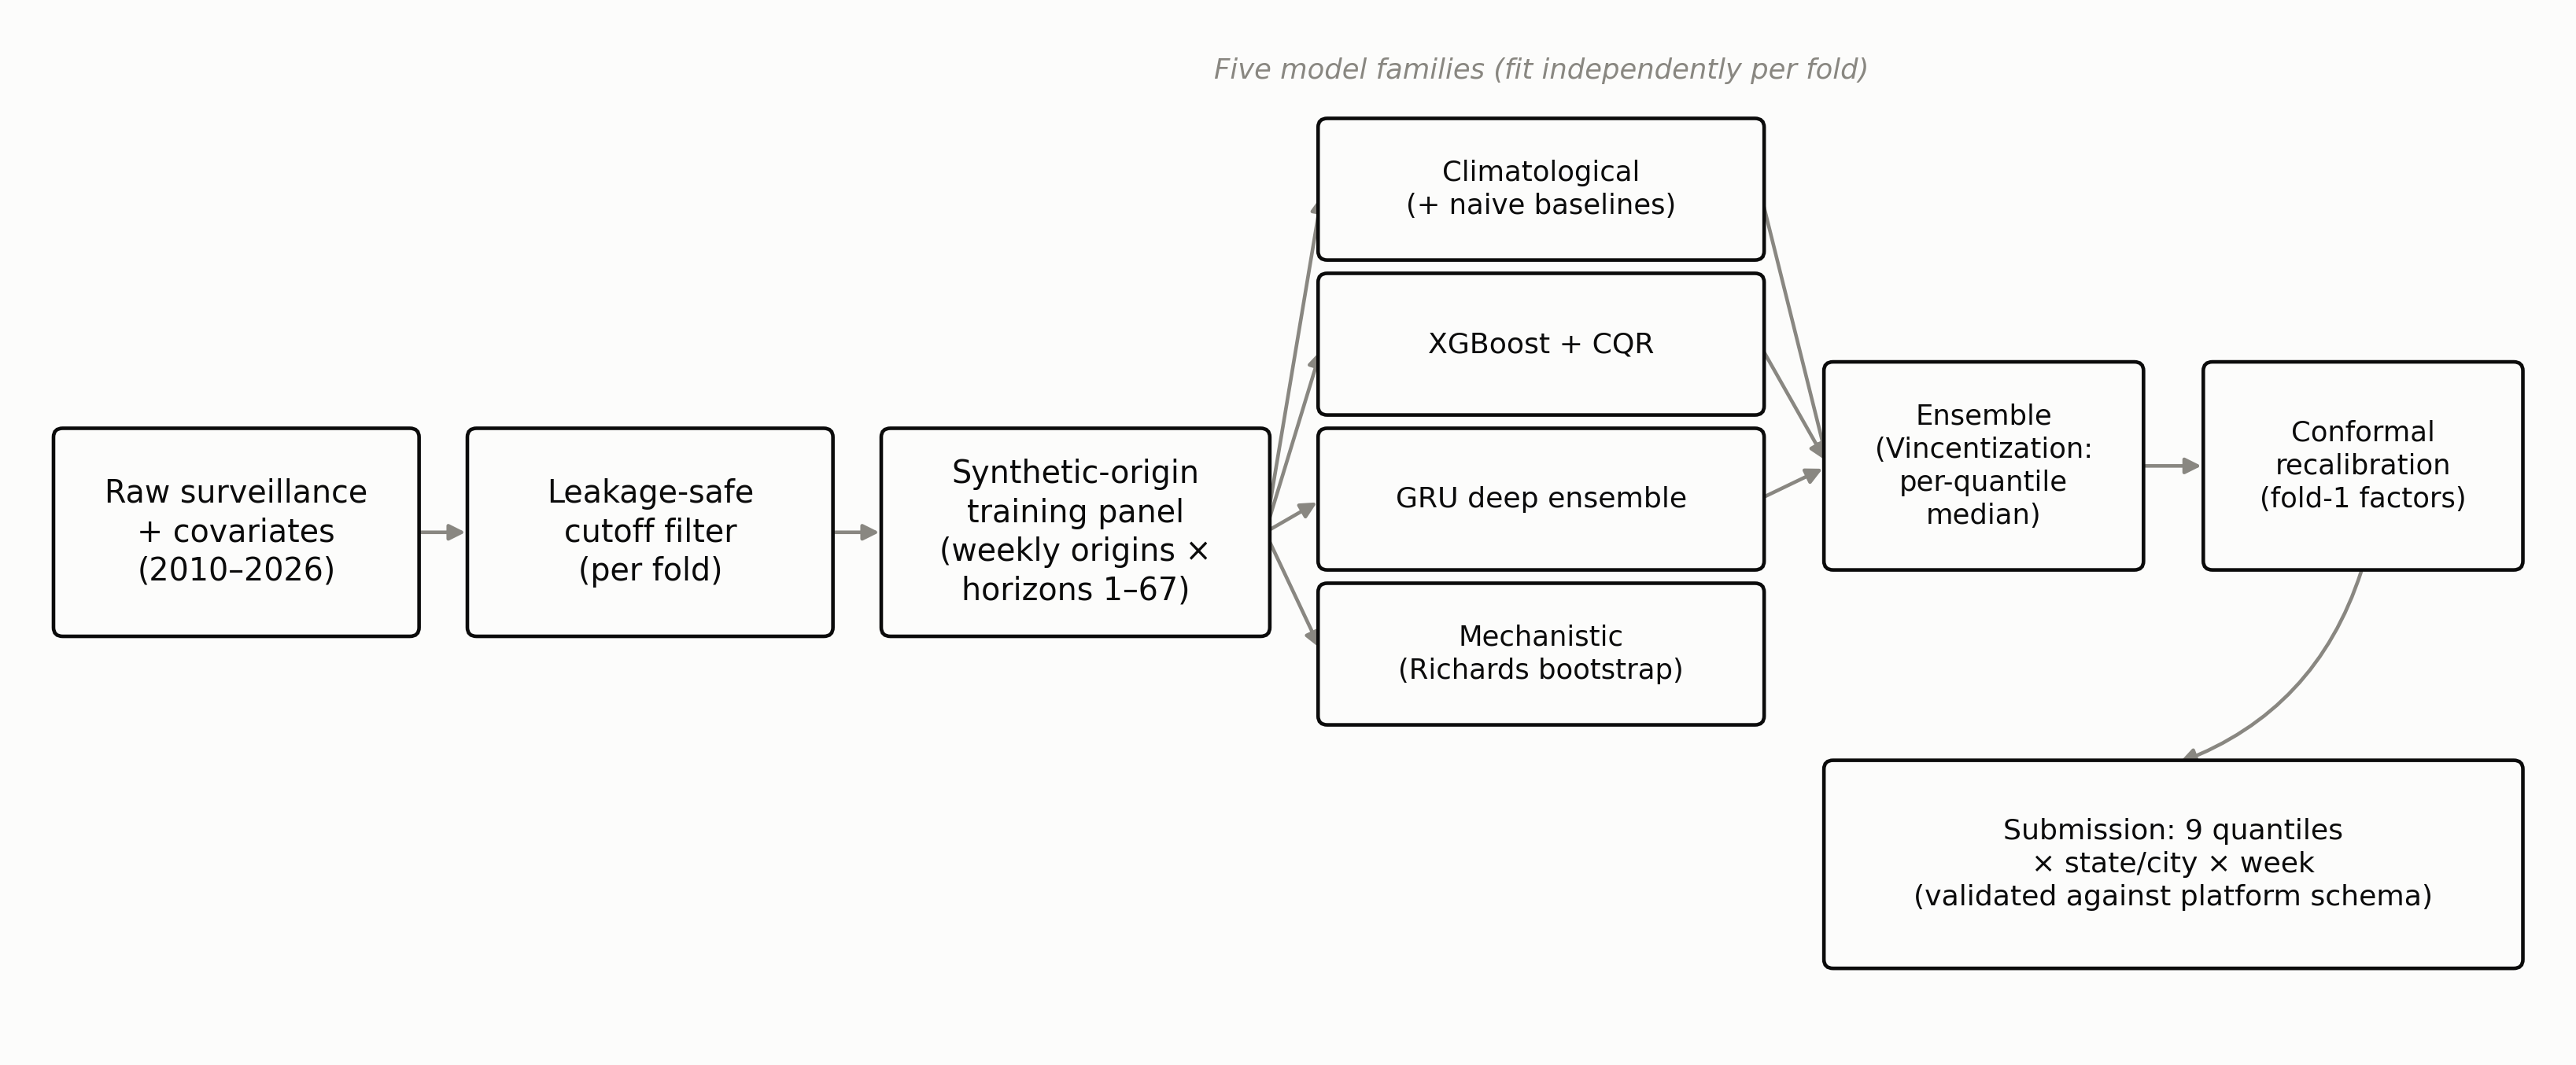
\includegraphics[width=0.98\textwidth]{../results/figures/paper_pipeline.png}
\caption{\textbf{Pipeline overview.} The dengue state-level pipeline, the most complex of the four
tracks: cutoff-filtered data becomes a synthetic-origin training panel, four model families are fit
independently, three of them (climatological, XGBoost, GRU) are combined by per-quantile median
into an ensemble, and conformal recalibration produces the final submitted quantiles. The mechanistic
model is evaluated for comparison but is not an ensemble member. Chikungunya-state and the city
tracks (not shown) follow the same stages but submit a single family's output directly.}
\label{fig:pipeline}
\end{figure}

\subsection{Data and targets}\label{sec:methods-data}
Weekly dengue and chikungunya case counts per municipality (2010--2026) are drawn from the Infodengue
system, which harmonizes notifiable-disease surveillance \citep{codeco2018}, and aggregated to the 26
mandatory states, excluding Espírito Santo per the challenge. Covariates comprise weekly climate
reanalysis (temperature, precipitation, humidity, pressure, thermal range, rainy days), a seasonal
climate forecast, ocean-oscillation indices (El Ni\~no--Southern Oscillation, Indian Ocean Dipole,
Pacific Decadal Oscillation), yearly municipal population, and static climate-zone and biome
covariates. The forecasting target is the weekly state case count over each season, submitted as the
nine quantiles 0.025, 0.05, 0.10, 0.25, 0.50, 0.75, 0.90, 0.95, and 0.975.

\subsection{Backtest design and leakage control}\label{sec:methods-backtest}
The four official seasons are derived at runtime from the challenge's train and target flags. A
confirmed 15-week gap separates each training cutoff from the start of its evaluation window,
simulating reporting delay. Two leakage disciplines are enforced centrally in the harness rather than
in individual models. All covariate access is filtered to dates at or before the training cutoff, and
lag and rolling features are computed from the continuous cutoff-filtered history rather than from the
gapped target window. Both are checked by automated regression tests, so a leak would fail the test
suite rather than silently inflate scores.

\subsection{Scoring}\label{sec:methods-scoring}
Forecasts are scored by the weighted interval score,
\[
\mathrm{WIS}(F,y)=\frac{1}{K+\tfrac12}\Big[\tfrac12\,|y-m|+\sum_{k=1}^{K}\frac{\alpha_k}{2}\,
\mathrm{IS}_{\alpha_k}(\ell_k,u_k,y)\Big],
\]
over the four required central intervals, where $m$ is the predictive median, $\mathrm{IS}_{\alpha}$
is the interval score at level $1-\alpha$ (the interval's width plus a penalty, scaled by $2/\alpha$,
for however far the observation falls outside it), and the weights reproduce the mean pinball loss
over the
nine required quantiles, the exact discrete approximation to the continuous ranked probability score
\citep{gneiting2007,bracher2021}. Concretely, for a simplified two-interval version of the score with median $m=10$, a
50 percent interval $[6,14]$, a 90 percent interval $[2,20]$, and an observation $y=15$: the median
term is $\tfrac12|15-10|=2.5$; the 50 percent interval ($\alpha=0.5$) is exceeded by 1 (since
$15>14$), giving
$\mathrm{IS}_{0.5}=(14-6)+\tfrac{2}{0.5}(15-14)=12$, weighted by $\alpha/2=0.25$ to $3$; the 90
percent interval ($\alpha=0.1$) is not exceeded, giving $\mathrm{IS}_{0.1}=(20-2)=18$, weighted by
$0.05$ to $0.9$;
so, with $K=2$ intervals, $\mathrm{WIS}=(2.5+3+0.9)/(2+0.5)=2.56$. Our implementation is verified
against this hand-computed
value, against an independent pinball-loss re-derivation, and against the challenge platform's own
scorer. We also report empirical interval coverage, a decomposition of WIS into dispersion and
directional (over- and under-prediction) penalties, a scale-free per-unit relative WIS, and the
normalized WIS (sum of WIS divided by sum of observed cases) that the challenge adopts as its headline
metric.

\subsection{Models}
\textbf{Baselines.} A naive model (last observed value with empirical horizon-difference quantiles), a
seasonal-naive model (same-epidemiological-week history), and a climatological quantile model (direct
order-statistic quantiles per state and epidemiological week over a five-week window).

\noindent\textbf{Gradient boosting.} Only four official evaluation windows exist per disease, far
too few to fit a tree ensemble, so a gradient-boosted quantile model is instead fit on a
synthetic-origin panel: within each fold's own cutoff-filtered history, every Sunday from roughly
2014 onward becomes a candidate forecast origin, and every (origin, horizon) pair from 1 to 67 weeks
ahead becomes one training row, with origin-anchored lag, rolling, seasonal, climate, ocean,
seasonal-forecast, and static features as inputs and the realized case count that many weeks later
as the label. For example, one row might read: origin = the first Sunday of March 2021, horizon = 12
weeks, features computed using only data available on that March Sunday, label = the observed case
count 12 weeks after it. This turns roughly 500 usable weekly origins per state, crossed with up to
67 horizons, into tens of thousands of training rows for a single fold, while evaluation still only
ever happens at that fold's own four-times-a-year official target window. We evaluated two
gradient-boosting implementations on this identical panel: LightGBM \citep{ke2017}, one booster per
quantile level, and XGBoost \citep{chen2016}, a single booster with a native multi-quantile
objective covering all nine levels jointly. XGBoost scored significantly better both overall and on
the outlier season (Sections~\ref{sec:noseason} and \ref{sec:significance}) and is the version used
in the main ensemble; LightGBM remains the gradient-boosted family used for the chikungunya-state
track, on which it was not re-evaluated against XGBoost. Predictive intervals for both are
calibrated by conformalized quantile regression (CQR) \citep{romano2019}: a held-out slice of the
training panel is used to measure how much each quantile needs to be shifted so that it achieves its
nominal coverage, and that shift is then applied to the model's raw quantile predictions, in the
same spirit as, but computed independently from, the ensemble-level conformal recalibration of
Section~\ref{sec:methods-conformal}.

\noindent\textbf{Deep learning.} A global gated recurrent unit (GRU) network \citep{cho2014}, a type
of recurrent neural network designed to retain information over many time steps, with
per-state embeddings and a negative-binomial output head (chosen over a Poisson head because case
counts are more variable than a Poisson distribution allows), trained as a deep ensemble of
independently seeded runs \citep{lakshminarayanan2017}; quantiles are analytic, meaning computed
directly from the fitted negative-binomial distribution's formula rather than by simulation, and
pooled across ensemble members by quantile averaging.

\noindent\textbf{Semi-mechanistic.} A model that bootstraps historical season trajectories under a
negative-binomial observation model. Trajectories come from a local reimplementation of
Richards-curve epidemic-scanner fits \citep{richards1959}: the Richards curve is a flexible,
S-shaped growth-then-plateau curve long used to summarize an epidemic's rise and fall, fit
separately to each historical season, from which we resample plausible future trajectories. Because
it draws on the full spread of past seasons rather than assuming a fixed noise scale, this
produces wide, well-calibrated intervals under distribution shift.

\noindent\textbf{Ensembles.} Models are combined by per-quantile median (Vincentization) and,
separately, by inverse-WIS weights: each model's weight is proportional to $1/\overline{\mathrm{WIS}}$
on the designated tuning season, so a model that scored better on that season counts for more,
tuned only on the designated tuning season, so weights are never fit on the
seasons on which the ensemble is reported.

\subsection{Conformal recalibration}\label{sec:methods-conformal}
Section~\ref{sec:conformal} gives a worked numeric example of this procedure's effect on one
interval; here we give the full definition. For each central interval level $L$ with bounds
$[\ell_L,u_L]$ and median $m$, we compute a
multiplicative widening factor $s_L$ that makes the interval reach its nominal coverage on the tuning
season. For each calibration unit, the multiple needed to just cover the observation is
$r=(y-m)/(u_L-m)$ when $y>m$ and $r=(m-y)/(m-\ell_L)$ when $y<m$; $s_L$ is the $L/100$ empirical
quantile of $r$, a scale-free, multiplicative analogue of conformalized quantile regression that is
robust to the large cross-state differences in scale. The interval is then widened about the median
by $s_L$, and monotonicity across quantiles is restored by a rearrangement step. Factors are estimated
on the tuning season and applied to all seasons; recalibrating the ensemble output outperforms
recalibrating any single member. The same frozen, fold-1-derived factors are reused unchanged for the
forecast phase, consistent with fitting recalibration weights only once and never on the season being
forecast.

\subsection{Reproducibility}
All code, the backtesting harness, per-state scored predictions, and validated submission files for
four official tracks (dengue and chikungunya, state and city level) are released. The pipeline is
deterministic under a fixed seed, and an automated test suite covers leakage safety, scoring
correctness, model persistence, and every model family. A provenance manifest records the exact data
and code state behind each reported number. The Supporting Information provides the full feature list
and frozen hyperparameters, the deep-learning architecture, the mechanistic derivation, per-state and
per-fold tables, the ensemble-member and weight robustness analysis, and an item-by-item EPIFORGE 2020
reporting checklist \citep{pollett2021}.

\section*{Data and code availability}
The pipeline was developed by team Neural Earth for the 3rd Infodengue--Mosqlimate Dengue Challenge.
All code, data-processing pipeline, backtests, figures, and validated submissions are openly available
at \url{https://github.com/kamrul28890/3rd_imdc_purdue_neuralearth}. The surveillance and covariate
data are distributed by the challenge through the Mosqlimate platform.

\section*{Author contributions}
Conceptualization, methodology, software, formal analysis, investigation, visualization, and writing
of the original draft: M.K.K. Validation, data curation, and writing (review and editing): E.J.E. and
A.A.H. All authors read and approved the final manuscript.

\section*{Competing interests}
The authors have declared that no competing interests exist.

\section*{Funding}
The authors received no specific funding for this work.

\section*{Ethics statement}
This study used aggregate, publicly available disease-surveillance and covariate data distributed
through the Infodengue and Mosqlimate platforms. No individual-level data were used and no ethical
approval was required.

\section*{AI usage}
Development of the analysis pipeline, statistical methods, code, and portions of this manuscript
was assisted by Claude (Anthropic), an AI assistant, under the direction and review of the human
authors. All methodological decisions, interpretations, and conclusions are the responsibility of
the human authors, who reviewed and verified the code, analyses, and results.

\section*{Acknowledgments}
We thank the organizers of the Infodengue--Mosqlimate Dengue Challenge and the Infodengue and
Mosqlimate teams for curating and distributing the data.

\bibliographystyle{unsrtnat}
\begin{thebibliography}{99}
\small
\bibitem{araujo2026} Araujo EC, Carvalho LM, Coelho FC, et al. Leveraging probabilistic forecasts for dengue preparedness and control: the 2024 Dengue Forecasting Sprint in Brazil. \emph{Proc Natl Acad Sci USA} (2026).
\bibitem{carvalho2023} Carvalho LM, Villela DAM, Coelho FC, Bastos LS. Bayesian inference for the weights in logarithmic pooling. \emph{Bayesian Anal} 18(1):223--251 (2023).
\bibitem{bracher2021} Bracher J, Ray EL, Gneiting T, Reich NG. Evaluating epidemic forecasts in an interval format. \emph{PLoS Comput Biol} 17(2):e1008618 (2021).
\bibitem{gneiting2007} Gneiting T, Raftery AE. Strictly proper scoring rules, prediction, and estimation. \emph{J Am Stat Assoc} 102(477):359--378 (2007).
\bibitem{romano2019} Romano Y, Patterson E, Cand\`es EJ. Conformalized quantile regression. \emph{Adv Neural Inf Process Syst} 32 (2019).
\bibitem{gibbs2021} Gibbs I, Cand\`es EJ. Adaptive conformal inference under distribution shift. \emph{Adv Neural Inf Process Syst} 34 (2021).
\bibitem{ke2017} Ke G, Meng Q, Finley T, et al. LightGBM: a highly efficient gradient boosting decision tree. \emph{Adv Neural Inf Process Syst} 30 (2017).
\bibitem{chen2016} Chen T, Guestrin C. XGBoost: a scalable tree boosting system. \emph{Proc 22nd ACM SIGKDD Int Conf Knowledge Discovery and Data Mining} 785--794 (2016).
\bibitem{cho2014} Cho K, van Merri\"enboer B, Gulcehre C, et al. Learning phrase representations using RNN encoder-decoder for statistical machine translation. \emph{Proc EMNLP} (2014).
\bibitem{lakshminarayanan2017} Lakshminarayanan B, Pritzel A, Blundell C. Simple and scalable predictive uncertainty estimation using deep ensembles. \emph{Adv Neural Inf Process Syst} 30 (2017).
\bibitem{gasparrini2010} Gasparrini A, Armstrong B, Kenward MG. Distributed lag non-linear models. \emph{Stat Med} 29(21):2224--2234 (2010).
\bibitem{lowe2021} Lowe R, Lee SA, O'Reilly KM, et al. Combined effects of hydrometeorological hazards and urbanisation on dengue risk in Brazil. \emph{Lancet Planet Health} 5(4):e209--e219 (2021).
\bibitem{cramer2022} Cramer EY, Ray EL, Lopez VK, et al. Evaluation of individual and ensemble probabilistic forecasts of COVID-19 mortality in the United States. \emph{Proc Natl Acad Sci USA} 119(15):e2113561119 (2022).
\bibitem{reich2019} Reich NG, Brooks LC, Fox SJ, et al. A collaborative multiyear, multimodel assessment of seasonal influenza forecasting in the United States. \emph{Proc Natl Acad Sci USA} 116(8):3146--3154 (2019).
\bibitem{sherratt2023} Sherratt K, Gruson H, Grah R, et al. Predictive performance of multi-model ensemble forecasts of COVID-19 across European nations. \emph{eLife} 12:e81916 (2023).
\bibitem{pollett2021} Pollett S, Johansson MA, Reich NG, et al. Recommended reporting items for epidemic forecasting and prediction research: the EPIFORGE 2020 guidelines. \emph{PLoS Med} 18(10):e1003793 (2021).
\bibitem{johansson2019} Johansson MA, Apfeldorf KM, Dobson S, et al. An open challenge to advance probabilistic forecasting for dengue epidemics. \emph{Proc Natl Acad Sci USA} 116(48):24268--24274 (2019).
\bibitem{codeco2018} Codeço CT, Coelho F, Cruz O, et al. Infodengue: a nowcasting system for the surveillance of arboviruses in Brazil. \emph{Rev Saude Publica} (2018).
\bibitem{lowe2021b} Lowe R, et al. Nonlinear and delayed impacts of climate on dengue risk in Barbados. \emph{PLoS Med} 15(7):e1002613 (2018).
\bibitem{makridakis2020} Makridakis S, Spiliotis E, Assimakopoulos V. The M4 competition: 100,000 time series and 61 forecasting methods. \emph{Int J Forecast} 36(1):54--74 (2020).
\bibitem{colon2021} Col\'on-Gonz\'alez FJ, Sewe MO, Tompkins AM, et al. Projecting the risk of mosquito-borne diseases in a warmer and more populated world. \emph{Lancet Planet Health} 5(7):e404--e414 (2021).
\bibitem{richards1959} Richards FJ. A flexible growth function for empirical use. \emph{J Exp Bot} 10(2):290--301 (1959).
\bibitem{bhatt2013} Bhatt S, Gething PW, Brady OJ, Messina JP, et al. The global distribution and burden of dengue. \emph{Nature} 496:504--507 (2013).
\bibitem{messina2019} Messina JP, Brady OJ, Golding N, Kraemer MUG, et al. The current and future global distribution and population at risk of dengue. \emph{Nat Microbiol} 4:1508--1515 (2019).
\bibitem{desouza2023} de Souza WM, de Lima STS, Sim\~oes Mello LM, et al. Spatiotemporal dynamics and recurrence of chikungunya virus in Brazil: an epidemiological study. \emph{Lancet Microbe} 4(5):e319--e329 (2023).
\bibitem{gneiting2014} Gneiting T, Katzfuss M. Probabilistic forecasting. \emph{Annu Rev Stat Appl} 1:125--151 (2014).
\bibitem{zaffran2022} Zaffran M, F\'eron O, Goude Y, Josse J, Dieuleveut A. Adaptive conformal predictions for time series. \emph{Proc 39th Int Conf Machine Learning (PMLR)} 162 (2022).
\bibitem{held2005} Held L, H\"ohle M, Hofmann M. A statistical framework for the analysis of multivariate infectious disease surveillance counts. \emph{Stat Model} 5(3):187--199 (2005).
\bibitem{meyer2017} Meyer S, Held L, H\"ohle M. Spatio-temporal analysis of epidemic phenomena using the R package surveillance. \emph{J Stat Softw} 77(11):1--55 (2017).
\bibitem{imdc2026webinar} Infodengue-Mosqlimate Dengue Challenge. IMDC 2026 Validation Round: First-Phase Results (webinar). 31 July 2026. \url{https://www.youtube.com/watch?v=m96WaySHznw}.
\end{thebibliography}

\end{document}
